\section{Le stage}
\subsection{Les missions}
J'ai été recruté comme stagiaire chez SHERPA Engineering afin d'apporter une aide à l'intégration et aux tests terrain pour compte du défi 3 du Challenge MOBILEX*.\\\\
\indent Ma mission principale consiste à participer aux tests des différentes briques logicielles développées sur le robot. Les tests se font d'abord en simulation, puis, lorsque les résultats sont concluants, sur le terrain. Lors des tests terrains, il est nécessaire de prévoir une série de tests pertinents pour mettre à l'épreuve les briques sous test et de communiquer avec l'équipe de l'INRAE pour programmer une date et prévoir la disponibilité du matériel à utiliser pour les tests. Une fois les tests réalisés, un compte-rendu est fait à l'équipe de développement.\\\\
\indent En cas de problèmes lors des tests, il est impératif de noter les circonstances dans lesquelles ils sont apparus, trouver des scénarios reproduisant ces derniers, réaliser des diagnostics, isoler la cause et, dans la mesure du possible, proposer une solution de résolution.\\\\
\indent En dehors des sessions de tests planifiées, mes missions se sont articulées autour de deux axes principaux : \\

\begin{itemize}
\renewcommand{\labelitemi}{$\bullet$}
    \item \textbf{L'automatisation du post-traitement} : J'ai développé un générateur automatique de rapports d'essais. Cet outil synthétise les données d'exécution afin de fournir une analyse visuelle et rapide du déroulement des tests.
    \item \textbf{La standardisation des procédures} : J'ai mis sur pied un protocole et un plan de test rigoureux. Ce cadre méthodologique vise d'une part à évaluer la conformité du système vis-à-vis des exigences fonctionnelles spécifiées par la DGA pour le Défi 3, et d'autre part à garantir la répétabilité des scénarios d'essai, indépendamment de l'ingénieur chargé de l'exécution.\\
\end{itemize}
    
\indent Enfin, j'ai travaillé sur l'amélioration de la fonctionnalité de suivi de lisière en y intégrant une prise en compte des obstacles sur le chemin.


\subsection{Présentation des travaux réalisés}

\subsubsection{Prise en main du projet}
Lors de mon arrivée à SHERPA Engineering, il a été indispensable pour moi de prendre en main un projet débuté depuis plus de deux ans.\\\\
\indent Mon premier objectif a consisté à cloner le dépôt Git de l'ensemble du projet Mobiter sur notre poste de travail. Ce dernier fonctionne sous Ubuntu 22.04 et intègre Distrobox, un outil de conteneurisation permettant d'exécuter une surcouche logicielle sous un autre système d'exploitation — en l'occurrence Ubuntu 20.04. Cette configuration est indispensable pour utiliser ROS Noetic. En effet, l'intégralité de la brique logicielle MOBILEX a été développée sous cette version de ROS, qui s'avère incompatible avec la distribution native Ubuntu 22.04. \\\\
\indent Une fois le simulateur fonctionnel, j'ai alors pu me familiariser avec l'utilisation de l'IHM et les différents modes de conduite disponibles. Puis afin de pouvoir proposer des tests pertinents et comprendre l'architecture logicielle de la brique MOBILEX*, aussi bien d'un point de vue théorique que technique, il m'a fallut consulter l'ensemble des codes.

\subsubsection{Migration et évaluation du SLAM (Simultaneous Localization and Mapping)}

La pile logicielle (stack) MOBITER nécessite une estimation de pose précise et continue. Si la disponibilité permanente du GNSS RTK lors du défi 1 garantissait ces conditions, l'introduction de coupures GNSS temporaires lors du défi 2 ($< 2\text{ min}$) a imposé l'intégration d'une solution alternative. Un algorithme de SLAM LiDAR (\textbf{Kitware}), couplé à une extrapolation IMU pour augmenter la fréquence d'échantillonnage, a été déployé conjointement avec un module d'arbitrage chargé d'assurer la transition entre les sources de localisation. Bien que fonctionnelle pour le défi 2, cette architecture a révélé deux limitations majeures : \\

\begin{itemize}
    \item \textbf{Une dérive spatiale critique} : Fortement dépendante de la structure géométrique de l'environnement, la dérive intrinsèque du SLAM kitware engendrait des discontinuités de pose (sauts de localisation) trop importantes lors de la réacquisition du signal GNSS. Pour prévenir tout comportement instable, le module d'arbitrage interdisait le basculement si l'écart mesuré dépassait un seuil critique, contraignant le robot à poursuivre sa navigation en mode SLAM dégradé jusqu'à la fin de la mission.
    \item \textbf{Une charge computationnelle élevée} : Le SLAM de Kitware constituait le processus le plus budgétivore en ressources calcul de la stack, risquant d'induire des verrous de performance avec l'ajout de nouvelles fonctionnalités.\\
\end{itemize}

Face à l'allongement prévisible des masquages GNSS lors du défi 3, le SLAM LiDAR de Kitware a été remplacé par l'approche \textbf{DLIO*} (Direct LiDAR-Inertial Odometry), caractérisée par une dérive significativement plus faible. Parallèlement, un gestionnaire de discontinuité de localisation a été ajouté pour faire face à la discontinuité de pose lors des transitions SLAM$\rightarrow$GNSS, garantissant le réengagement du GNSS RTK quelle que soit la dérive cumulée tout en maintenant le suivi du scénario.\\

\begin{comment}
Au début de mon stage, l'équipe Mobiter avait engagé des travaux de refonte du module de SLAM (Simultaneous Localization and Mapping). Lors des défis précédents, la solution logicielle reposait exclusivement sur le Kitware SLAM, une approche purement LiDAR. Celle-ci présentait de graves limites dans les environnements très dégagés (comme les grands espaces extérieurs), où la rareté des caractéristiques géométriques et des retours LiDAR nuisait à la qualité de la localisation. De plus, ce composant représentait l'une des charges computationnelles les plus lourdes de la pile logicielle du projet. Afin de pallier ces défauts, le SLAM DLIO (Direct LiDAR-Inertial Odometry), combinant les données LiDAR et une centrale inertielle (IMU), a été choisi comme une alternative plus robuste pour la navigation en milieux ouverts.\\\\ 
\end{comment}

\indent C’est dans ce contexte du défi 3 que j'ai participé à l'évaluation et aux tests du SLAM DLIO en simulation et sur terrain au sein de la brique MOBILEX*. Une fois son intégration logicielle finalisée, nous avons mené une campagne de tests afin de valider son bon fonctionnement et de quantifier ses performances (en matière de dérive et de charge CPU) par rapport au Kitware SLAM et à la vérité terrain.


\paragraph{Fonctionnement du Kitware SLAM}

Le \textbf{Kitware SLAM} repose sur l'algorithme LOAM* (\textit{LiDAR Odometry And Mapping in Real-time}) \cite{LOAM}, qui se décompose en trois étapes principales :

\subparagraph{a. Le prétraitement et l'extraction des caractéristiques géométriques du nuage de points LiDAR}:

La première étape consiste à prétraiter le nuage de points LiDAR afin d'atténuer les distorsions subies lors du mouvement du véhicule pendant l'acquisition, puis d'extraire les éléments géométriques nécessaires au recalage. Contrairement aux approches traitant l'intégralité des points du scan, LOAM sélectionne uniquement les points présentant une information géométrique forte. Cette sélection réduit la charge computationnelle tout en préservant les contraintes physiques indispensables à l'estimation de pose. Deux types de caractéristiques sont principalement extraits :\\

\begin{itemize}
    \item \textbf{Les points d'arêtes (\textit{edge features}) :} ils correspondent aux zones présentant une forte variation de courbure (angles de bâtiments, contours d'obstacles).
    \item \textbf{Les points plans (\textit{surface features}) :} ils identifient les zones de faible variation de courbure, représentatives de surfaces régulières (sol, murs, façades).\\
\end{itemize}

Ces caractéristiques sont ensuite exploitées lors des phases de recalage afin de calculer la transformation rigide entre deux acquisitions successives.

\subparagraph{b. L'estimation de l'odométrie LiDAR}:

La deuxième étape vise à évaluer le déplacement relatif du robot entre deux scans consécutifs. Pour cela, LOAM réalise un recalage \textbf{scan-to-scan} entre les caractéristiques extraites de l'acquisition courante et celles de la précédente. L'estimation de la transformation spatiale est obtenue par la minimisation de deux métriques d'erreur :\\
 
\begin{itemize}
    \item Une distance point-droite pour les caractéristiques d'arêtes.
    \item Une distance point-plan pour les caractéristiques de surface.\\
\end{itemize}  

L'optimisation sous ces contraintes fournit la transformation à une fréquence supérieure à celle de la cartographie. Néanmoins, ce traitement reste sujet à la dérive par accumulation des erreurs de recalage.

\subparagraph{c. La construction de la carte et l'optimisation spatiale}:

La troisième étape reconstruit progressivement la carte globale de l'environnement tout en corrigeant la dérive accumulée par l'odométrie. À l'inverse de l'étape précédente, le recalage s'effectue cette fois entre le scan courant et la carte locale (\textbf{scan-to-map}). Les caractéristiques du nouveau nuage de points sont alignées avec la carte préexistante afin d'affiner l'estimation de pose, garantissant ainsi la cohérence spatiale à long terme.\\

Bien que la documentation détaillée du \textbf{Kitware SLAM} soit restreinte, cet algorithme intègre un système d'optimisation par graphe de poses \cite{kitware_slam}, capable de réajuster l'ensemble de la carte lors d'une fermeture de boucle (\textbf{loop closure}). Il propose également une extraction enrichie de caractéristiques, incluant la détection de ruptures d'intensité lumineuse ou d'amas de points (\textbf{blobs}).
De plus, le module offre la possibilité d'injecter des données exogènes issues d'autres capteurs (IMU, GNSS, INS, odométrie des roues, caméras RGB pour balises visuelles). Toutefois, les essais expérimentaux menés n'ont pas révélé de gain de performance significatif lors de l'intégration directe de l'IMU au sein du SLAM. Cela a justifié le choix de conserver (dans le cadre du défi 2) une version exclusivement LiDAR pour le SLAM et de coupler l'IMU de manière externe afin d'élever la fréquence de la localisation. Enfin, certaines fonctionnalités avancées ont dû être restreintes afin d'assurer le respect des contraintes temps réel de la pile logicielle (\textbf{stack}).


\paragraph{Fonctionnement du DLIO* SLAM}

DLIO* (Direct LiDAR-Inertial Odometry) \cite{dlio_slam} est un algorithme d'odométrie LiDAR-inertielle sobre en calcul et conçu pour maintenir une localisation précise et construire une carte 3D dense même lors de mouvements agressifs ou dans des environnements peu structurés. Contrairement aux approches fondées sur l'extraction de primitives géométriques (LOAM, Kitware SLAM) et le recalage intermédiaire \textbf{scan-to-scan}, DLIO adopte une approche directe opérant directement sur le nuage de points dense. Il réalise un recalage direct \textbf{scan-to-map} grace aux garanties de convergence formelles de son observateur d'état. Son traitement repose sur quatre étapes clés :

\subparagraph{a. Prétraitement et conditionnement des données denses}:

La première étape consiste à réaliser un alignement spatio-temporel des données LiDAR ($10\text{--}20\text{ Hz}$) et IMU ($100\text{--}500\text{ Hz}$) dans le repère du robot sans sous-échantillonnage agressif (par grille de voxel) ni extraction de primitives (arêtes, plans, etc.). Sur le nuage de points dense est appliqué un simple filtrage spatial de proximité destiné à éliminer les points appartenant à la structure propre du robot. L'algorithme offre aussi la possibilité d’ajouter un léger sous-échantillonnage (0.05 à 0.1m) pour les LiDARs très denses.
    
\subparagraph{b. Correction de mouvement}:

Pendant la durée du balayage LiDAR, les mouvements du robot induisent des distorsions spatiales importantes. Pour éliminer ces déformations sans recourir aux simplifications classiques (vitesse constante) ni au coût de calcul élevé d’autres méthodes d’interpolation, DLIO introduit une approche séquentielle de type \textbf{coarse-to-fine} \cite{coarse_to_fine} décrite comme suit :\\

\begin{itemize}
    \item \textbf{Coarse step} : Les mesures IMU comprises entre deux scans LiDAR successifs sont intégrées numériquement sous l’hypothèse d’un modèle de mouvement d’ordre supérieur à secousse linéaire et accélération angulaire constantes. Cela permet d’obtenir une estimation de l’état du robot à chaque nouvelle valeur IMU.
    \item \textbf{Fine step} : Pour chaque point du nuage acquis à l’instant relatif $t_n$, DLIO se sert des deux états estimés par l’IMU encadrant $t_n$ pour résoudre un jeu d’équations analytiques sous forme close paramétré uniquement par l’horodatage $t_n$. Ce calcul exact et parallélisable corrige la distorsion (\textbf{deskewing}) et projette le nuage dans le repère monde $\mathcal{W}$, générant une estimation de l'état \textit{a priori} $\hat{\mathbf{T}}_{\text{prior}}^{\mathcal{W}}$ pour le recalage géométrique.\\
\end{itemize}
    
\subparagraph{c. Recalage géométrique (GICP* : Generalized Iterative Closest Point)}:

Grâce à la précision de l'estimation initiale, DLIO s'affranchit du recalage scan-to-scan et effectue directement un alignement scan-to-map. Le nuage corrigé $\hat{\mathcal{P}}_k^{\mathcal{W}}$ est aligné sur une sous-carte locale $\hat{\mathcal{S}}_k^{\mathcal{W}}$ constituée d'images-clés (keyframes). Cet alignement s'appuie sur l'algorithme GICP \cite{gicp}, qui modélise la surface locale par des matrices de covariance et minimise la distance de Mahalanobis (correspondance plan-à-plan). L'optimisation produit la transformation $\Delta \hat{\mathbf{T}}_k$, affinant ainsi la pose globale $\hat{\mathbf{T}}_k^{\mathcal{W}}$.

\subparagraph{d. Fusion et mise à jour d'état}: 

Pour fusionner les données LiDAR et IMU, DLIO intègre un observateur géométrique non linéaire hiérarchique. Il combine la pose affinée par le GICP aux mesures IMU haute fréquence afin d'estimer l'état complet du système :

\begin{equation}
    \hat{\mathbf{x}}_k = \begin{bmatrix} \mathbf{p}^{\mathcal{W}} & \mathbf{q}^{\mathcal{W}} & \mathbf{v}^{\mathcal{W}} & \mathbf{b}_a & \mathbf{b}_\omega \end{bmatrix}^\top
\end{equation}
représentant respectivement la position, l'orientation, la vitesse et les biais de l'IMU.\\
\indent Fondé sur la théorie de la contraction, cet observateur garantit une convergence globale théorique. Les états estimés sont réinjectés dans les intégrations IMU ultérieures, fermant ainsi la boucle d'estimation.


\paragraph{Comparaison expérimentale DLIO vs Kitware SLAM}

Afin de comparer la qualité de la localisation des 2 SLAM, nous avons mené une série de tests expérimentaux sur différents terrains. Sur une trajectoire de 320 mètres réalisée dans un environnement naturel relativement riche en obstacles (\hyperref[fig27]{Figure 27}), nous avons obtenu les parcours présenté en annexe \hyperref[annexe5]{[INRAE]} et les courbes suivantes (\hyperref[fig28]{Figure 28} et \hyperref[fig29]{Figure 29}) représentant les positions et orientations estimées par chaque SLAM par rapport à la vérité terrain donnée par le GNSS RTK.\\

\begin{center}
    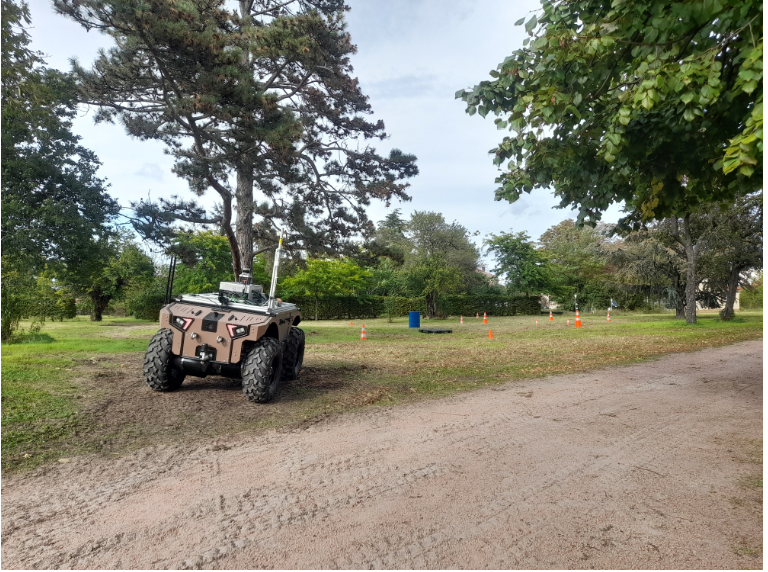
\includegraphics[width=0.5\linewidth]{Corps_rapport/inrae.png}
    \captionof{figure}{Terrain d’essais de l’INRAE Aubière}
    \label{fig27}
\end{center}

\begin{figure}[h]
    \centering
    \begin{subfigure}[b]{0.48\textwidth}
        \centering
        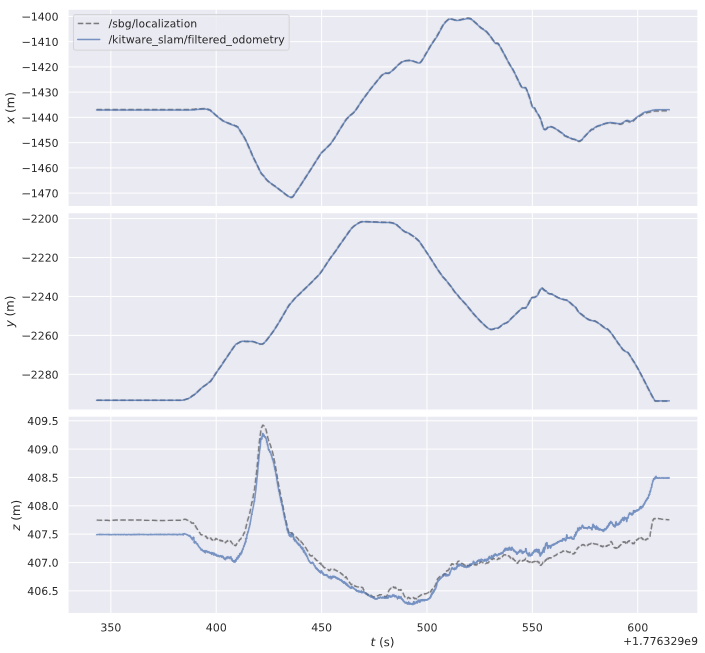
\includegraphics[width=\textwidth]{Corps_rapport/kitware_position_inrae.png}
        \caption{position évaluée par kitware}
        \label{fig:image1}
    \end{subfigure}
    \hfill
    \begin{subfigure}[b]{0.48\textwidth}
        \centering
        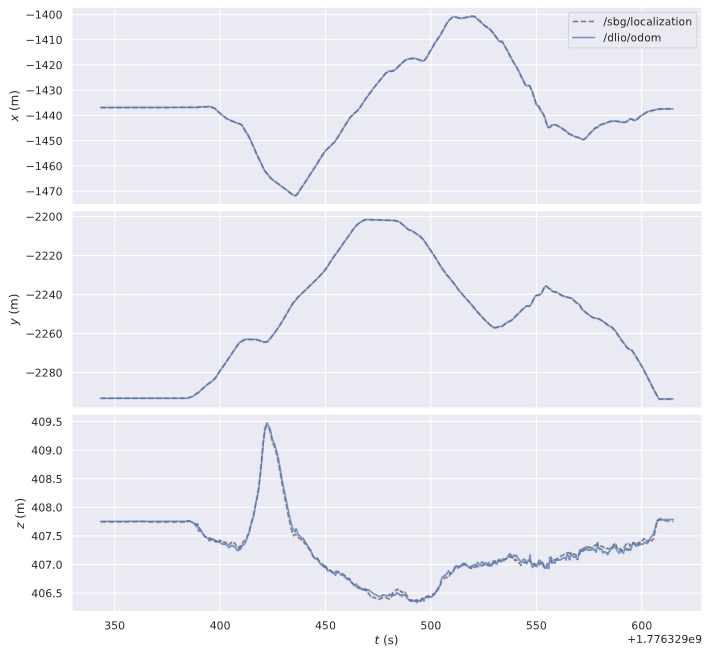
\includegraphics[width=\textwidth]{Corps_rapport/dlio_position_inrae.png}
        \caption{position évaluée par DLIO}
        \label{fig:image2}
    \end{subfigure}    
    \caption{Comparaison des positions Kitware vs DLIO vs vérité terrain}
    \label{fig28}
\end{figure}

\begin{figure}[h]
    \centering
    \begin{subfigure}[b]{0.48\textwidth}
        \centering
        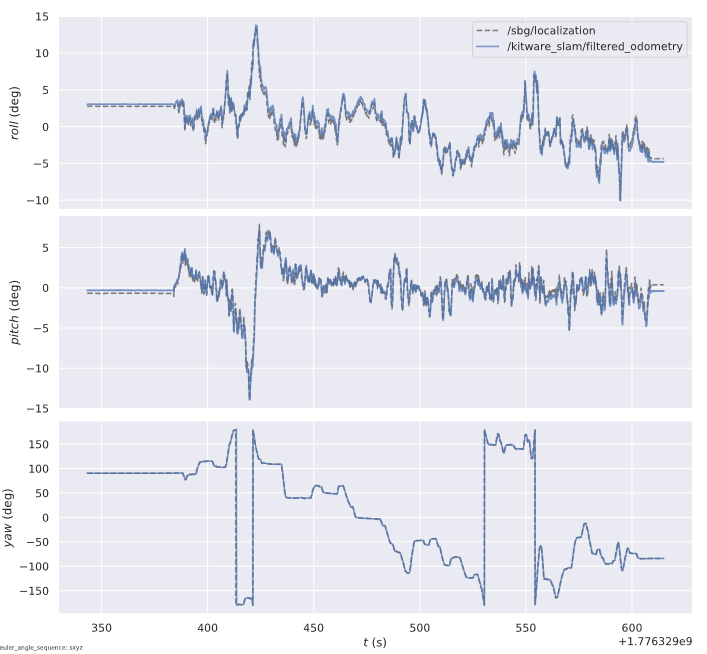
\includegraphics[width=\textwidth]{Corps_rapport/kitware_RPY_inrae.png}
        \caption{orientation évaluée par kitware}
        \label{fig:image1}
    \end{subfigure}
    \hfill
    \begin{subfigure}[b]{0.48\textwidth}
        \centering
        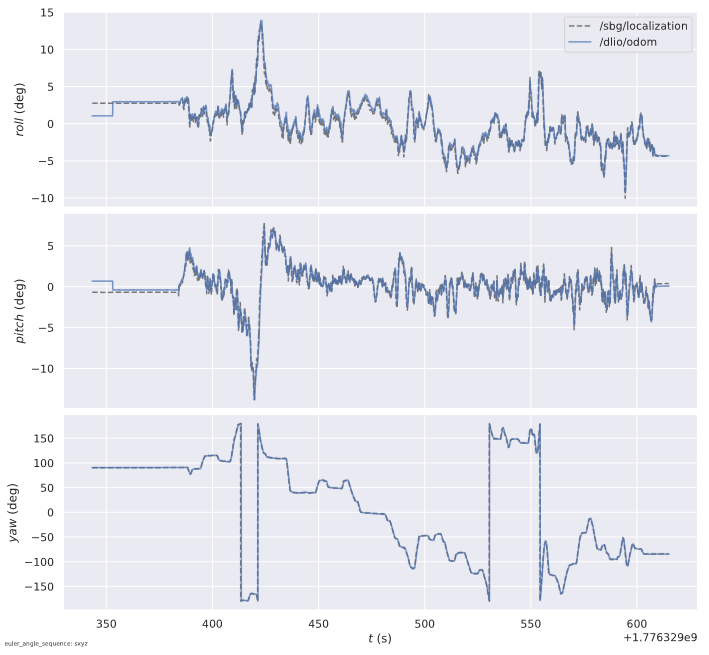
\includegraphics[width=\textwidth]{Corps_rapport/dlio_RPY_inrae.png}
        \caption{orientation évaluée par DLIO}
        \label{fig:image2}
    \end{subfigure}    
    \caption{Comparaison des orientations Kitware vs DLIO vs vérité terrain}
    \label{fig29}
\end{figure}

Au regard des courbes précedentes, on peut constater que les 2 SLAM offrent en environnement structuré des trajectoires alignées avec la vérité terrain. Cependant, le SLAM DLIO présente des erreurs de pose bien plus faible que le SLAM Kitware comme le témoigne la figure (\hyperref[fig30]{Figure 30}) ci-dessous.

\begin{center}
    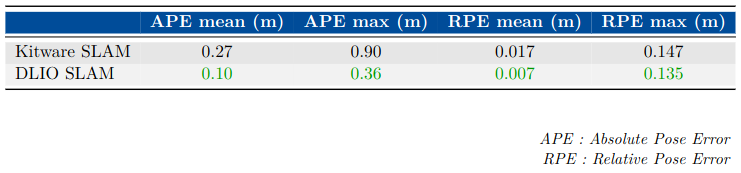
\includegraphics[width=1.0\linewidth]{Corps_rapport/Kitware_vs_dlio_metrics.png}
    \captionof{figure}{Comparaison des erreurs de pose sur le terrain d’essais de l’INRAE Aubière}
    \label{fig30}
\end{center}

Puis sur une plus longue trajectoire de près de 1 km réalisée dans un environnement naturel fortement dégagé (\hyperref[fig31]{Figure 31}), nous avons obtenu les parcours présenté en \hyperref[fig32]{Figure 32} représentant les poses estimées par chaque SLAM par rapport à la vérité terrain donnée par le GNSS RTK.\\

\begin{center}
    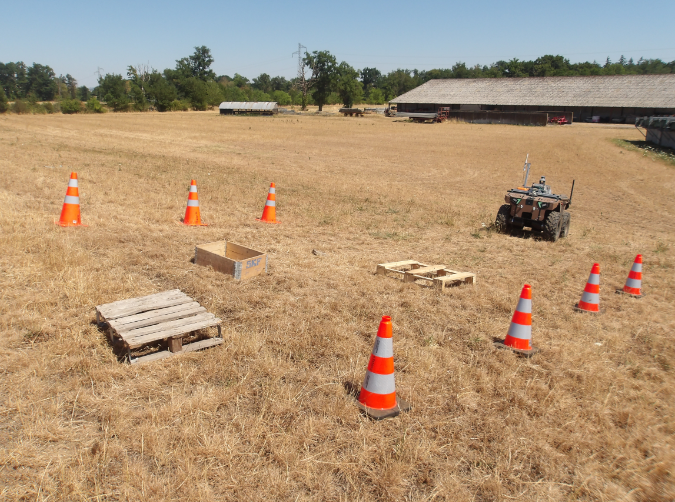
\includegraphics[width=0.5\linewidth]{Corps_rapport/montoldre.png}
    \captionof{figure}{Terrain d’essais de Montoldre}
    \label{fig31}
\end{center}

\begin{center}
    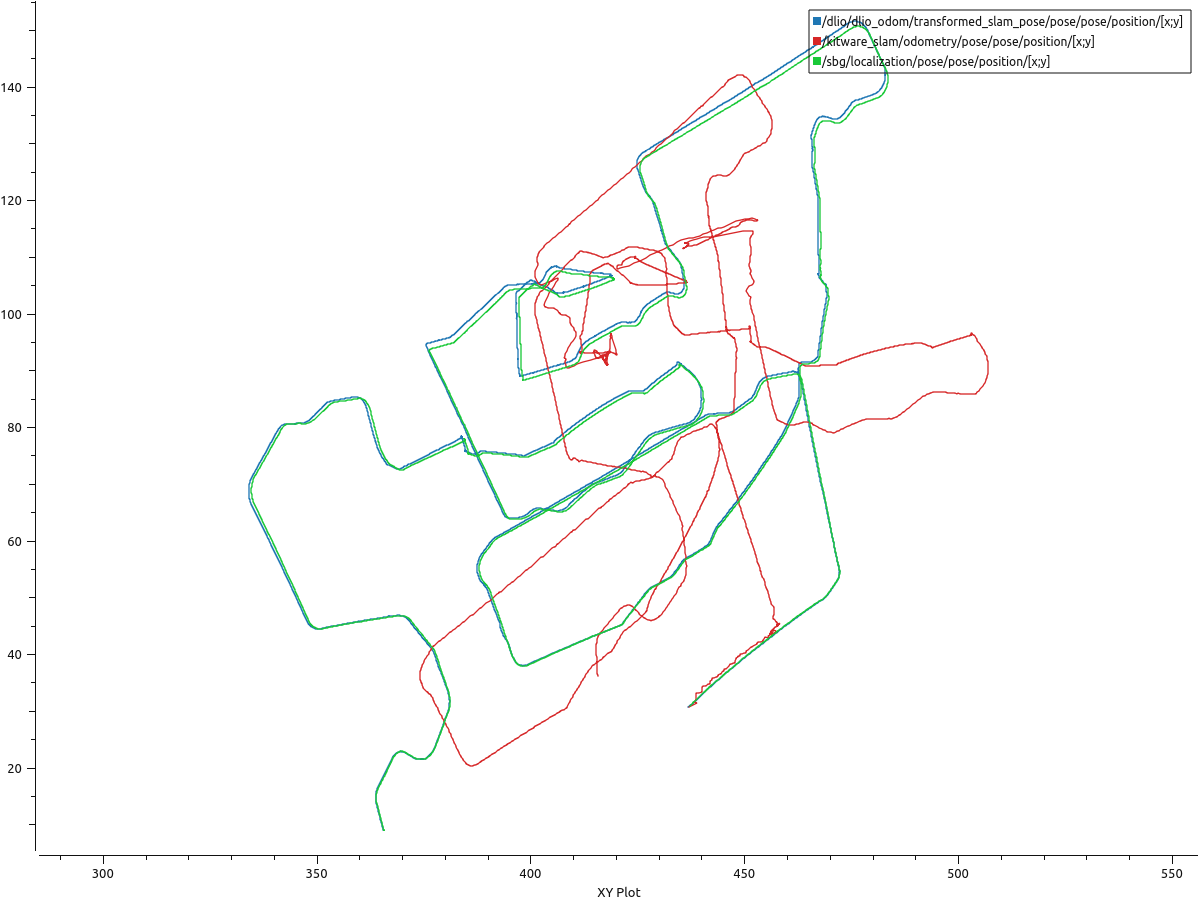
\includegraphics[width=0.8\linewidth]{Corps_rapport/dlio_vs_kitware_vs_Sbg_montoldre.png}
    \captionof{figure}{Comparaison des trajectoires DLIO vs Kitware vs vérité terrain en zone dégagée}
    \label{fig32}
\end{center}

Au regard de la figure précedente, on constate que le SLAM DLIO, grâce à son couplage inertiel-LiDAR, garantit une très bonne localisation, même en milieu dégagé. Ce n'est pas le cas du SLAM Kitware, qui montre des limites évidentes dans ces conditions. De plus, comme le montre l'annexe \hyperref[annexe6]{[montoldre]}, le SLAM DLIO présente une erreur de position maximale d'environ 1,5 mètre, tandis que celle du SLAM Kitware atteint environ 80 mètres d'erreur maximale sur ce parcours de 1 km. Enfin, on observe une réduction d’environ 50\% d’utilisation de RAM et de charge CPU avec le SLAM DLIO par rapport à notre version allégée de Kitware. Ces résultats confortent notre choix de changer de SLAM dans le cadre du défi 3.\\


\paragraph{Modifications apportées à DLIO SLAM}

Pour atteindre les performances illustrées précédemment, des modifications ont été apportées dans le code de base de DLIO. Initialement, DLIO donnait une dérive globale certes plus faible que le Kitware SLAM mais très bruité, rendant son exploitation dans la stack impossible sans dégrader la carte (\hyperref[fig33]{Figure 33}).

\begin{center}
    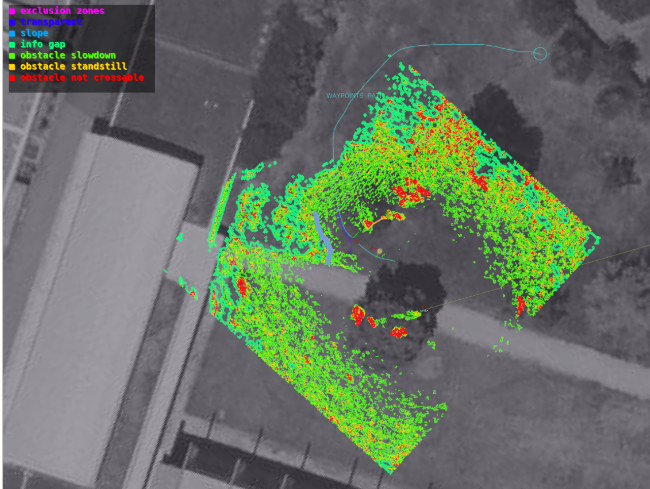
\includegraphics[width=0.5\linewidth]{Corps_rapport/map_dlio_bruit.png}
    \captionof{figure}{Carte construite avec la version originale de DLIO SLAM}
    \label{fig33}
\end{center}

Après avoir tenté d'atténuer ce bruit en ajustant les paramètres de l'observateur géométrique sans résultat concluant, une incohérence conceptuelle a été identifiée au sein du code du SLAM : \textbf{les fusions entre les observations LiDAR et IMU n'étaient pas cohérentes temporellement}.\\

Considérons $t_{\text{scan}}$ le timestamp du dernier scan LiDAR, $t_{\text{gicp}}$ le temps de calcul nécessaire au recalage GICP du scan courant sur la carte locale, et $t_{\text{now}}$ le timestamp de l'état courant (associé à la dernière fusion IMU). Dans l'implémentation originale de DLIO, la durée $t_{\text{gicp}}$ était négligée. Le résultat du recalage GICP (correspondant à la pose à $t_{\text{scan}}$) était ainsi fusionné avec un état ayant déjà évolué durant $t_{\text{gicp}}$ pour atteindre $t_{\text{now}} \approx t_{\text{scan}} + t_{\text{gicp}}$. En raison de ce décalage temporel, l'observateur géométrique calculait un écart artificiellement élevé qu'il tentait de corriger, ce qui tirait l'état du robot vers une pose passée et perturbait l'estimation des vitesses (\textit{twists}) ainsi que des biais de l'IMU.\\

Pour résoudre ce problème, un tampon (\textit{buffer}) des états fusionnés par l'observateur a été implémenté et son fonctionnement a été repensé :
\begin{itemize}
    \item \textbf{Interpolation temporelle :} Le \textit{buffer} permet d'interpoler l'état exact à l'instant $t_{\text{scan}}$ afin d'y fusionner l'observation LiDAR.
    \item \textbf{Rétropropagation :} Comme l'état continue d'évoluer pendant la phase de recalage, les mesures IMU acquises entre $t_{\text{scan}}$ et $t_{\text{now}}$ sont rejouées (rétropropagées) à partir de l'état à $t_{\text{scan}}$ corrigé par le GICP, remplaçant ainsi l'état \textit{a priori} à $t_{\text{now}}$.\\
\end{itemize}

Cette correction a permis d'accorder un poids supérieur au recalage GICP dans l'observateur, autorisant des corrections plus franches tout en réduisant la dérive globale.\\

Enfin, une dérive anormale observée en sortie de l'observateur par rapport aux résultats bruts du GICP a été résolue en substituant l'IMU intégrée du LiDAR Ouster ($100\text{ Hz}$), particulièrement bruitée, par l'IMU de la Xsens ($100\text{ Hz}$) moin bruitée. Voire annexe \hyperref[annexe7]{[pose\_gicp]} pour plus de détails. Ces modifications intégrées ont permis d'obtenir une carte de meilleure qualité et une dérive globale plus faible, comme le montre la figure ci-dessous (\hyperref[fig34]{Figure 34}).

\begin{center}
    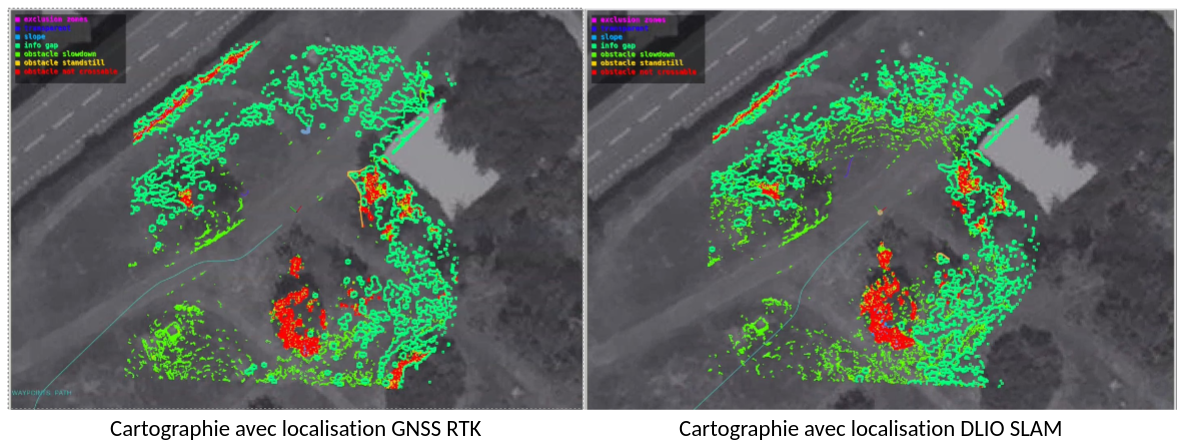
\includegraphics[width=1\linewidth]{Corps_rapport/Comparaison_map_DLIO_vs_GNSS.png}
    \captionof{figure}{Comparaison de cartographie en GNSS RTK VS en DLIO}
    \label{fig34}
\end{center}

\indent Comme le montre la figure ci-dessus, la carte générée par le SLAM DLIO est de bonne qualité et garantit une navigation fiable lorsqu'on la compare à la vérité terrain fournie avec le GNSS RTK. L'étape suivante a consisté à évaluer la dérive du SLAM DLIO par rapport à la vérité terrain en fonction de la distance parcourue.

\begin{comment}
Nous avons par la suite évalué les performances du SLAM DLIO en comparant sa trajectoire à la vérité terrain ainsi qu'à celle générée par le SLAM Kitware. C'est dans cette optique que des essais ont été menés sur les sites de l'INRAE d'Aubière et de Montoldre. La méthodologie a consisté, dans un premier temps, à enregistrer un fichier de données (rosbag) lors d'un déplacement en téléopération avec le SLAM DLIO actif, tout en enregistrant la position de référence renvoyée par la centrale de navigation SBG. Dans un second temps, ce bag a été rejoué hors ligne afin d'exécuter le SLAM Kitware et de générer un fichier unique centralisant les trois sources de localisation (GNSS RTK, DLIO et Kitware). Enfin, l'utilisation des outils de la bibliothèque EVO nous a permis de comparer et d'évaluer précisément les performances des deux algorithmes de SLAM par rapport à la vérité terrain (\hyperref[fig27]{Figure 27} et \hyperref[fig28]{Figure 28}).\\
\end{comment}


\subsubsection{Évaluation de la dérive du SLAM DLIO par rapport à la vérité terrain}

La bibliothèque python EVO, très employée pour l'évaluation de techniques de SLAM, utilise l'algorithme de Kabsch-Umeyama \cite{Kabsch} pour aligner les trajectoires avant comparaison et évaluation. Cet algorithme permet de trouver la meilleure transformation rigide (rotation et translation) qui minimise l'écart quadratique moyen (RMSD) entre deux ensembles de points appariés. Il est utile pour l'alignement d'ensembles de points en infographie, ainsi qu'en chimio-informatique et en bio-informatique pour comparer des structures moléculaires et protéiques. \\\\
\indent Cette étape de transformation est cruciale pour s'assurer que les trajectoires sont comparées dans le même référentiel, éliminant ainsi les effets de décalage initial ou de rotation. Une fois les nuage de points alignés, EVO compare les trajectoires et retourne les métriques suivantes: \\

\begin{itemize}
\renewcommand{\labelitemi}{$\bullet$}
    \item \textbf{max}: c'est la valeur de l'erreur la plus élevée enregistrée sur l'ensemble de la trajectoire.
    \item \textbf{mean}: c'est la moyenne arithmétique simple de toutes les erreurs de pose calculées.
    \item \textbf{median}: c'est la valeur centrale. Exactement la moitié des poses ont une erreur inférieure à la médiane, et l'autre moitié a une erreur supérieure.
    \item \textbf{min}: c'est la valeur de l'erreur la plus faible enregistrée sur l'ensemble de la trajectoire.
    \item \textbf{rmse} (Root Mean Square Error - Erreur Quadratique Moyenne): c'est la racine carrée de la moyenne des carrés des erreurs.
    \item \textbf{sse} (Sum of Squared Errors - Somme des Erreurs Quadratiques): c'est la somme de toutes les erreurs individuelles élevées au carré.
    \item \textbf{std} (Standard Deviation - Écart Type) : c'est une mesure de la dispersion des erreurs autour de la moyenne (mean).\\
\end{itemize}

\indent Afin de qualifier les performances du SLAM DLIO, il etait indispensable d'évaluer et visualiser sa dérive par rapport à la vérité terrain en fonction de la distance parcourue, chose qu'EVO ne permettait pas de faire. Pour cela, à partir d'un bag de données ROS contenant les trajectoires (SLAM et vérité terrain) enregistrées lors d'essais réels, nous avons implémenté un script qui calcule l'erreur euclidienne de position, la distance réelle parcourue puis la dérive du SLAM à chaque instant. La dérive étant donnée en pourcentage par la formule suivante \eqref{eq5}: 

\begin{equation} \label{eq5}
    \text{Dérive}[k] = \frac{100 \cdot \sqrt{(x_{\text{slam}}[k]-x_{\text{sbg}}[k])^2+(y_{\text{slam}}[k]-y_{\text{sbg}}[k])^2+(z_{\text{slam}}[k]-z_{\text{sbg}}[k])^2}}{\text{d}[k]}
\end{equation}
$\ $

avec $x_{\text{slam}}[k]$, $y_{\text{slam}}[k]$, $z_{\text{slam}}[k]$ les coordonnées de la position estimée par le SLAM à l'instant $k$, $x_{\text{sbg}}[k]$, $y_{\text{sbg}}[k]$, $z_{\text{sbg}}[k]$ les coordonnées de la vérité terrain fournie par la centrale SBG, et $\text{d}[k]$ la distance cumulée parcourue jusqu'à l'instant $k$, calculée de manière incrémentale selon la formule \eqref{eq6} : avec $\text{d}[0] = 0$.

\begin{equation} \label{eq6}
    \scalebox{0.9}{$\displaystyle\text{d}[k] = \text{d}[k-1] + \sqrt{(x_{\text{sbg}}[k]-x_{\text{sbg}}[k-1])^2+(y_{\text{sbg}}[k]-y_{\text{sbg}}[k-1])^2+(z_{\text{sbg}}[k]-z_{\text{sbg}}[k-1])^2}$}
\end{equation}
$\ $
 
\indent Une étape primordiale avant d'appliquer le calcul de la dérive consistait à s'assurer que les trajectoires SLAM et SBG (vérité terrain) soient dans le même repère et que, pour chaque instant $k$ (timestamp), les positions estimées par le SLAM et la vérité terrain soient appariées. Or, les deux trajectoires enregistrées dans le bag n'étaient pas parfaitement synchronisées ; nous avons donc dû les synchroniser en utilisant une fonction d'interpolation linéaire entre deux points successifs \eqref{eq7}. Cette fonction permet d'interpoler les données d'une trajectoire pour obtenir des valeurs correspondantes aux timestamps de l'autre trajectoire. Ainsi, nous avons pu aligner les deux ensembles de données et garantir que chaque position estimée par le SLAM correspondait à une position de vérité terrain à un instant donné.

\begin{equation} \label{eq7}
    f(t) = f(t_k) + \frac{t - t_k}{t_{k+1} - t_k} \cdot \bigl(f(t_{k+1}) - f(t_k)\bigr), \quad t_k \leq t \leq t_{k+1}
\end{equation}
$\ $

avec $f(t)$ la valeur interpolée à l'instant $t$, $t_k$ et $t_{k+1}$ les deux timestamps successifs encadrant $t$, et $f(t_k)$, $f(t_{k+1})$ les valeurs connues aux instants $t_k$ et $t_{k+1}$. Cette formule est appliquée indépendamment sur chaque coordonnée ($x$, $y$, $z$).\\

\indent La figure \hyperref[fig35]{Figure 35} illustre l'évolution de la dérive du SLAM DLIO par rapport à la vérité terrain en fonction de la distance parcourue. On observe que la dérive reste relativement faible, avec une valeur maximale d'environ 1,5\% sur l'ensemble de la trajectoire. Cette performance est significativement meilleure que celle du Kitware SLAM, qui présente une dérive plus importante, surtout dans les zones dégagées où les caractéristiques géométriques sont rares. Ces résultats confirment que le SLAM DLIO est une solution plus robuste et fiable pour la navigation en milieux ouverts, offrant une meilleure précision de localisation et une charge computationnelle réduite.\\ 

\begin{center}
    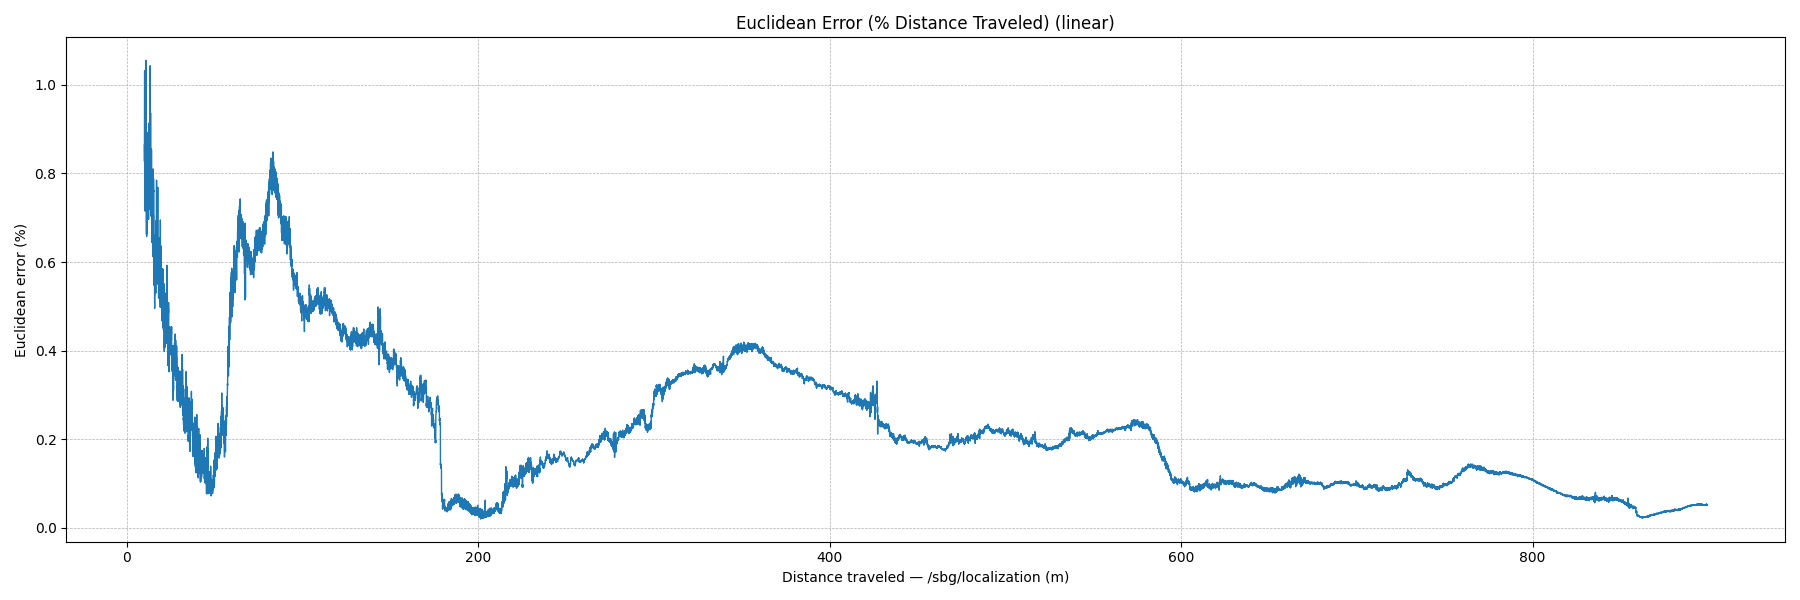
\includegraphics[width=1\linewidth]{Corps_rapport/euclidean_error_vs_distance.png}
    \captionof{figure}{Évolution de la dérive du SLAM DLIO par rapport à la vérité terrain en fonction de la distance parcourue}
    \label{fig35}
\end{center} 

Au regard de la figure ci-dessus, le SLAM DLIO présente une dérive particulièrement faible sur un parcours dégagé de 1 km, restant en dessous du seuil de 5 \% présenté par l'état de l'art dès 150 mètres parcourues. Ces résultats confirment définitivement son intégration pour la suite du challenge.\\

Afin d'évaluer l'adéquation des nouvelles fonctionnalités intégrées au module MOBILEX (notamment la navigation autonome reposant sur le SLAM DLIO) avec les exigences du défi 3 du challenge, un plan de test dédié a été conçu.

\subsubsection{Mise en place du plan de test}

Durant mon stage, il était attendu de moi la conception d'un plan de test rigoureux et reproductible afin d'évaluer les performances de la brique MOBILEX vis-à-vis des exigences du défi 3. Ce protocole vise à garantir la conformité des fonctionnalités du système avec les spécifications de la DGA, tout en assurant la répétabilité des essais, indépendamment de l'ingénieur chargé de leur exécution. Le terrain d'essais retenu pour le déroulement des tests est le site de l'INRAE Aubière du fait de sa proximité contrairement à celui de Montoldre. Il s'agissait ainsi de définir un ensemble de scénarios de test permettant la validation des exigences réglementaires fixées par la DGA (\hyperref[annexe3]{[règlementation DGA]}).\\

\indent À la suite d'échanges avec mon tuteur, nous avons opté pour le développement d'une carte géographique dynamique. Au sein de celle-ci, le positionnement des obstacles, des points de passage (waypoints) et des trajectoires s'adapte automatiquement au scénario sélectionné par l'opérateur. L'analyse topographique du terrain nous a permis d'identifier les zones propices au déroulement des différents essais. En nous appuyant sur des waypoints connus, nous avons délibérément choisi d'intégrer des obstacles (franchissables ou non) ainsi que des zones d'exclusion sur le site. Le résultat obtenu est illustré par la \hyperref[fig36]{Figure 36}.\\

\begin{center}
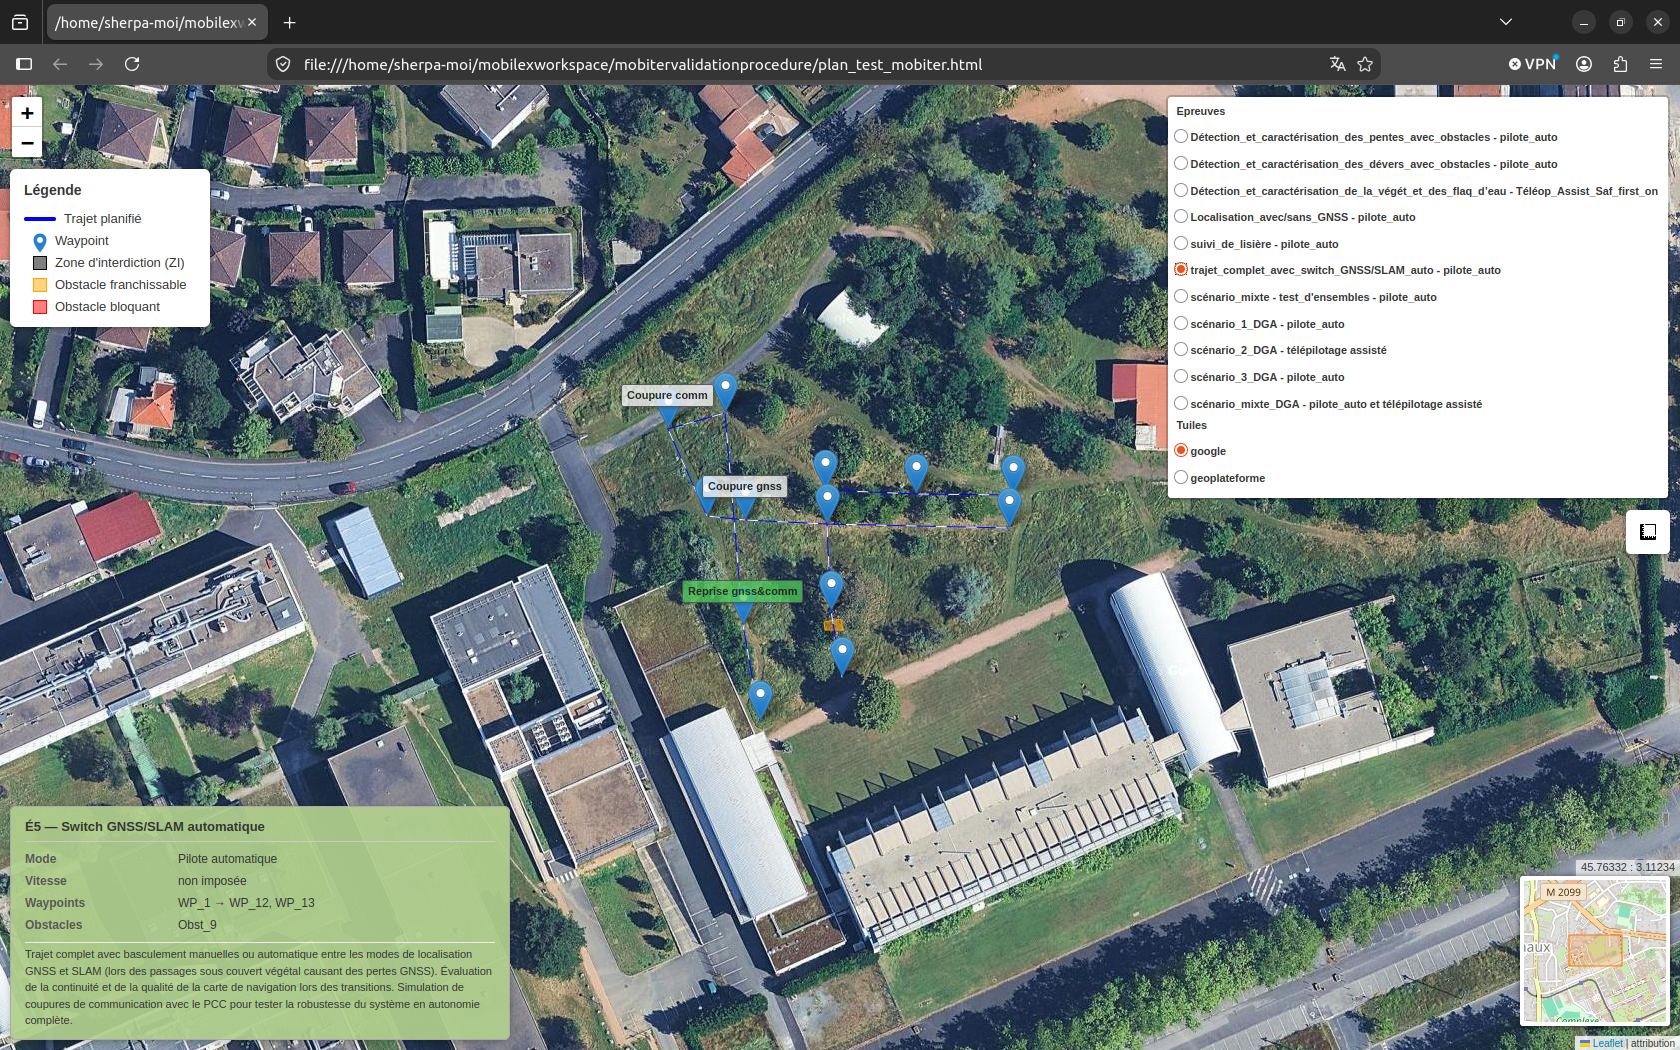
\includegraphics[width=1\linewidth]{Corps_rapport/plan_de_test_defi3.png}
\captionof{figure}{Plan de test graphique pour le défi 3}
\label{fig36}
\end{center} 

Cette carte dynamique a été développée en HTML et s'appuie sur la bibliothèque JavaScript Leaflet, dédiée à la création de cartes interactives. Elle permet de charger et d'afficher des données géospatiales issues de différentes sources, telles que des tuiles cartographiques ou des services de cartographie en ligne. L'interface utilisateur développée offre la possibilité de sélectionner divers scénarios de test ; la carte se met alors à jour automatiquement pour afficher les obstacles, les points de passage (waypoints) et les zones d'exclusion associés, tout en actualisant le descriptif de la mission dans la zone inférieure gauche.\\

\indent Une fois le plan de test graphique répétable établi, il a été nécessaire de mettre en place une checklist unique de propriétés à vérifier en ligne (lors du test) et hors ligne (après le test). Ce plan de test et cette checklist ont été conçus pour être utilisés par n'importe quel membre de l'équipe, garantissant ainsi la reproductibilité des tests et la comparaison des performances et résultats après chaque nouveau test. Elle comprend des points de contrôle précis subdivisé en 2 catégories: \\

\begin{itemize}
\renewcommand{\labelitemi}{$\bullet$}
    \item \textbf{Propriétés à vérifier en ligne} : Ces propriétés sont vérifiées en temps réel par l'opérateur lors de l'exécution du test. Elles incluent notamment la vérification de l'empatement du marquage au sol autour des waypoints, l'appui sur l'arrêt d'urgence durant le test, la reprise en téléopération du robot en cours de mission de suivi de waypoints, le ralentissement lors du franchissement d'obstacles ou de flaques d'eau ou de passage en mode SLAM, la perte de communication du robot avec le PCC, l'apparition d'accouts incessants lors du déplacement du robot et l'adéquation de la sémantique associée au retour vidéo de l'IHM avec l'environnement de test.
    \item \textbf{Propriétés à vérifier hors ligne} : Ces propriétés sont vérifiées après le test à partir des données enregistrées (ROS bag). Elles incluent notamment la vérification des trajectoires suivies par le robot, le respect des vitesses de commandes envoyées au robot, l'analyse de l'orientation (roll et pitch) du robot, et l'analyse des diagnostics émis sur l'IHM.\\
\end{itemize}

\indent Cette checklist présentée en annexe  \hyperref[annexe4]{[test\_checklist]} n'étant pas exhaustive, elle a été complétée par des points de contrôle pertinents supplémentaires en fonction des besoins et des observations faites lors des tests.\\

\indent Afin d'analyser efficacement les propriétés à vérifier hors ligne (après les essais), un générateur automatique de rapports a été développé. Cet outil synthétise les données d'exécution et fournit une analyse visuelle synthétique du déroulement des tests, facilitant ainsi le diagnostic et la prise de décision.\\

\subsubsection{Mise en oeuvre du générateur automatique de rapports d'essais}

L'une de mes missions principales a été de développer un générateur automatique de rapports d'essais. Cet outil vise à synthétiser les données d'exécution des tests pour fournir une analyse visuelle et rapide du déroulement des essais afin de faciliter les diagnostics.\\\\
\indent Le générateur de rapports d'essais a été conçu pour assurer un traitement offline des fichiers de données (ROS bag) enregistrés lors des tests. Il extrait les informations pertinentes, telles que les trajectoires, les vitesses, les erreurs de localisation, les événements critiques, les images de cartes construites et de visualisation, puis génère un rapport structuré comprenant des graphiques, des informations de diagnostic et des vidéos.\\\\
\indent Apres discussion avec l'ensemble de l'équipe, une liste d'éléments pertinents à inclure dans le rapport de test a été établie. Cette liste comprend notamment:\\

\begin{itemize}
\renewcommand{\labelitemi}{$\bullet$}
    \item La liste des diagnostics (avec timestamps) retournés sur l'IHM durant toute la durée des tests : sous forme de figure facilement interpretable puis sous forme de test plus descriptif contenant le message d'erreur associé à chaque disgnostic.
    \item Le mode de control du robot (téléopération, suivie de waypoint, ...) ainsi que le mode de localisation (GNSS, SLAM) du robot à chaque timestamps sous forme de figure.
    \item Un tracé des positions linéaires et angulaires du robot.
    \item Un tracé de la trajectoire du robot en slam et en GNSS RTK avec les waypoints à raliés, ainsi qu'une évaluation des erreurs de localisation.
    \item Un tracé de la trajectoire du robot avec les waypoints à raliés ainsi qu'une representation du mode de localisation sur chaque section de la trajectoire.
    \item Un tracé des erreurs de vitesses linéaires sur toute la tarjectoire par rapport aux vitesses de consigne souhaitée.
    \item Des vidéos synchronisées par rapport aux timestamps des bag, montrant la construction du MNE(Modele Numerique d'Elevation), de la planification globale, de la planification locale, de la carte des gradients ainsi que du retour vidéo sur l'IHM.\\
\end{itemize}

\indent L'outil a été développé en Python et utilise des bibliothèques telles que Matplotlib pour la visualisation des données, Pandas pour le traitement des données et OpenCV pour la manipulation d'images et de vidéos. A partir du bag ROS, le rapport final est généré au format html sous demande des membres de l'équipe. L'organigramme de l'outil est présenté dans la (\hyperref[fig37]{Figure 37}):\\

\begin{center}
    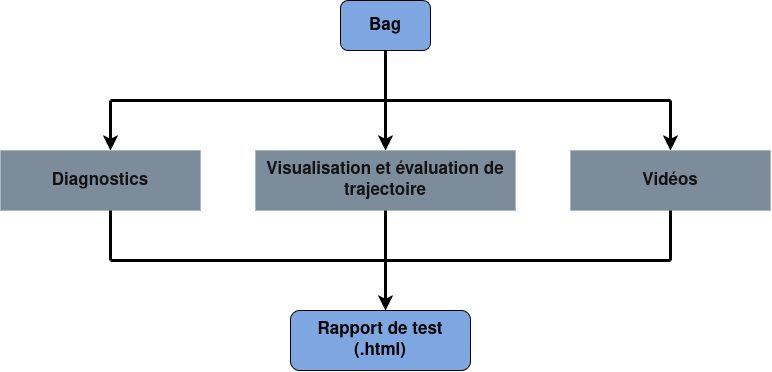
\includegraphics[width=0.8\linewidth]{Corps_rapport/org_bag_explorer.png}
    \captionof{figure}{Organigramme de l'outil de génération automatique de rapport de test}
    \label{fig37}
\end{center}

\paragraph{Extraction et génération des diagnostics de l'IHM}

L'objectif principal de ce module est d'obtenir une vision consolidée et exhaustive de l'ensemble des diagnostics émis par l'interface homme-machine (IHM) sur la totalité de la plage temporelle de l'essai. Cette approche permet notamment de capturer et de consigner les événements transitoires (des alertes fugaces qui apparaissent et disparaissent rapidement), évitant ainsi qu'ils ne soient omis par l'opérateur lors du déroulement du test en temps réel.\\

\indent Le processus débute par l'analyse du fichier d'enregistrement (bag file), dont l'objectif est d'extraire l'ensemble des topics de type \textbf{DiagnosticArray}. Si une liste restrictive de topics est fournie en paramètre, l'extraction se limite à ces derniers ; dans le cas contraire, l'intégralité des flux de type DiagnosticArray est récupérée par défaut. Une fois l'extraction effectuée, les informations utiles sont structurées et stockées chronologiquement au sein d'un dictionnaire indexé par horodatage (timestamp). À partir de cette structure de données, des scripts exploitant des library Python (pandas, numpy, matplotlib) génèrent automatiquement l'ensemble des figures d'analyse présentées précédemment, ainsi qu'un rapport de synthèse textuel (format .txt). De plus, afin de mettre en relation les anomalies matérielles ou logicielles avec l'état opérationnel du robot, l'outil extrait également les messages du topic \textbf{nav\_stack/control\_mux/mode}. L'analyse de ce topic permet de tracer et de corréler précisément les changements de modes de contrôle du système au cours de l'essai. Enfin, l'outil donne également un rapide aperçu des fréquences de publication des topics du bag par rapport celles de réference, permettant ainsi d'identifier les éventuels problèmes de communication ou de perte de données. La figure (\hyperref[fig38]{Figure 38}) suivante illustre l'organigramme de cet outil d'extraction de diagnostic:\\
 
\begin{center}
    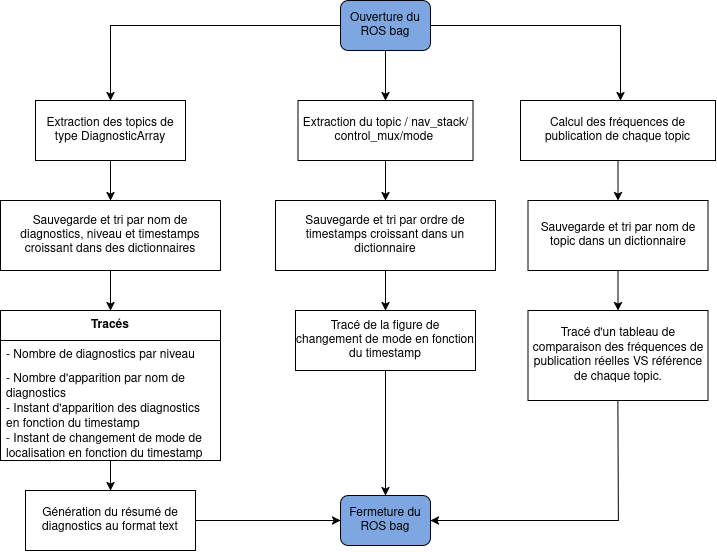
\includegraphics[width=0.7\linewidth]{Corps_rapport/org_diag_extractor.png}
    \captionof{figure}{Organigramme de l'outil d'extraction et de génération des diagnostics}
    \label{fig38}
\end{center}

\indent Comme résultat, l'outil génère plusieurs représentations graphiques, dont une frise chronologique (timeline) des diagnostics (\hyperref[fig39]{Figure 39}), indexée par identifiant d'alerte. Cette visualisation temporelle permet d'identifier immédiatement les éléments où des anomalies sont survenues, puis de fournir un résumé sur ces diagnostics anormaux détectés. Au sein de la pile logicielle (stack) MOBITER, les diagnostics sont hiérarchisés et catégorisés en quatre grands groupes fonctionnels (niveau) :\\

\begin{itemize}
\renewcommand{\labelitemi}{$\bullet$}
    \item \textbf{OK} : qui indique que tout fonctionne correctement.
    \item \textbf{WARNING} : qui indique un avertissement ou un problème potentiel.
    \item \textbf{ERROR} : qui indique une erreur nécessitant une attention immédiate.
    \item \textbf{STALE} : qui indique que les informations ne sont plus à jour.\\
\end{itemize}

\begin{center}
    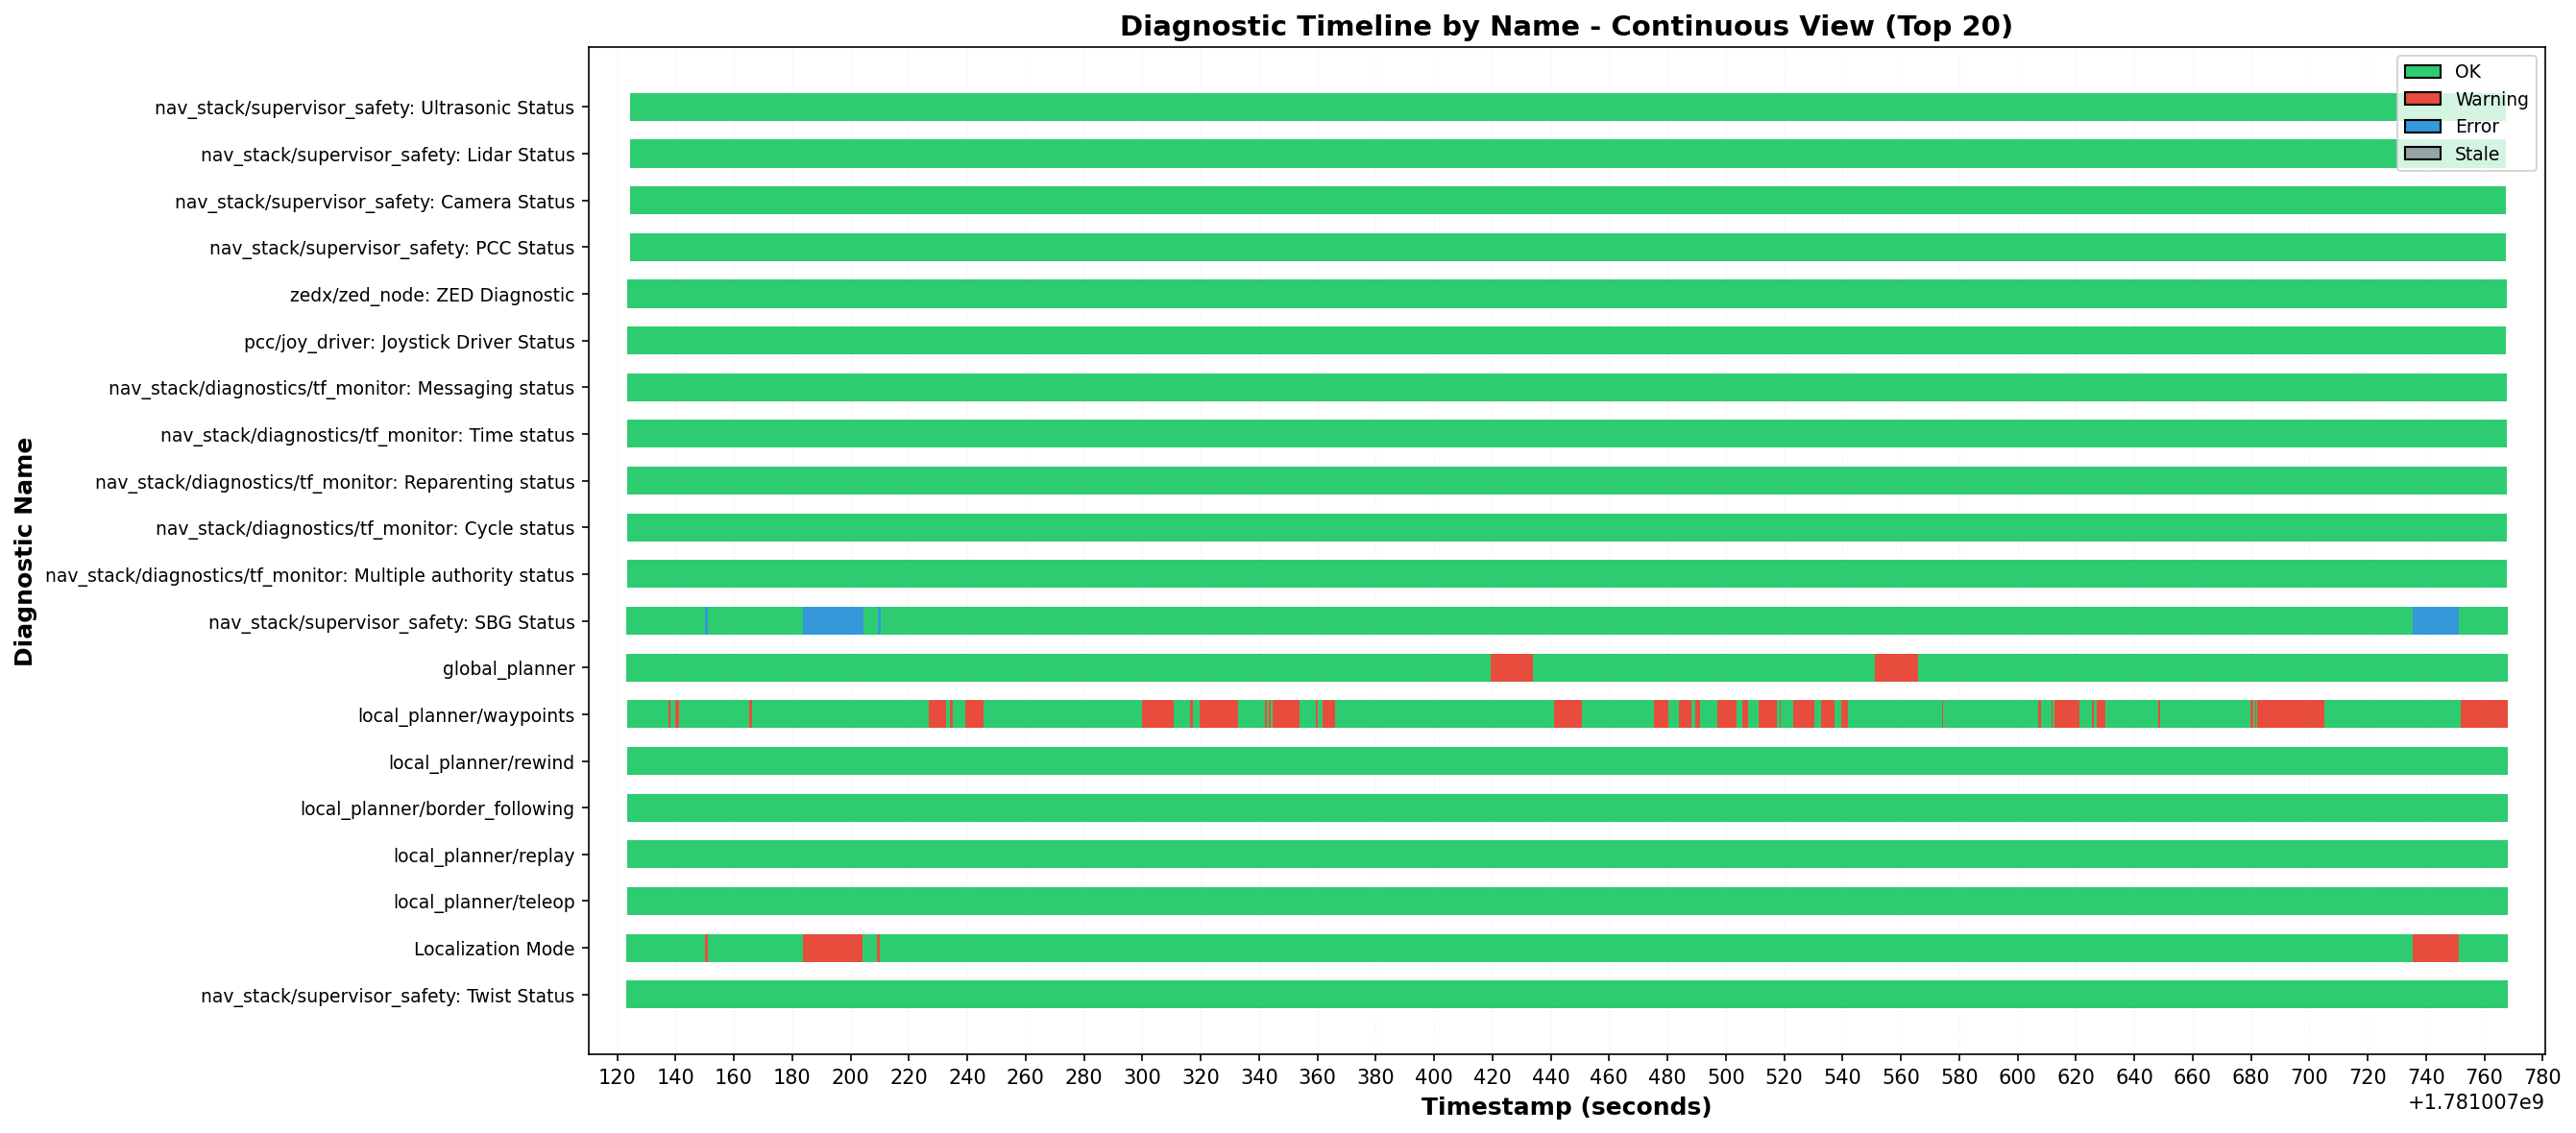
\includegraphics[width=1\linewidth]{Corps_rapport/diagnostics_timeline_by_name.png}
    \captionof{figure}{Timeline des diagnostics de l'IHM par nom de diagnostic}
    \label{fig39}
\end{center}

\indent Deplus, pour des soucis de débug il est souvent interessant de savoir à quel moment le robot a changé de mode de contrôle (téléopération, suivis de waypoint, suivis de lisiere) ou de localisation (GNSS ou SLAM). L'outil génère donc également des timelines de ces changements de mode de contrôle et de localisation (\hyperref[fig40]{Figure 40} et \hyperref[fig41]{Figure 41}).\\

\begin{center}
    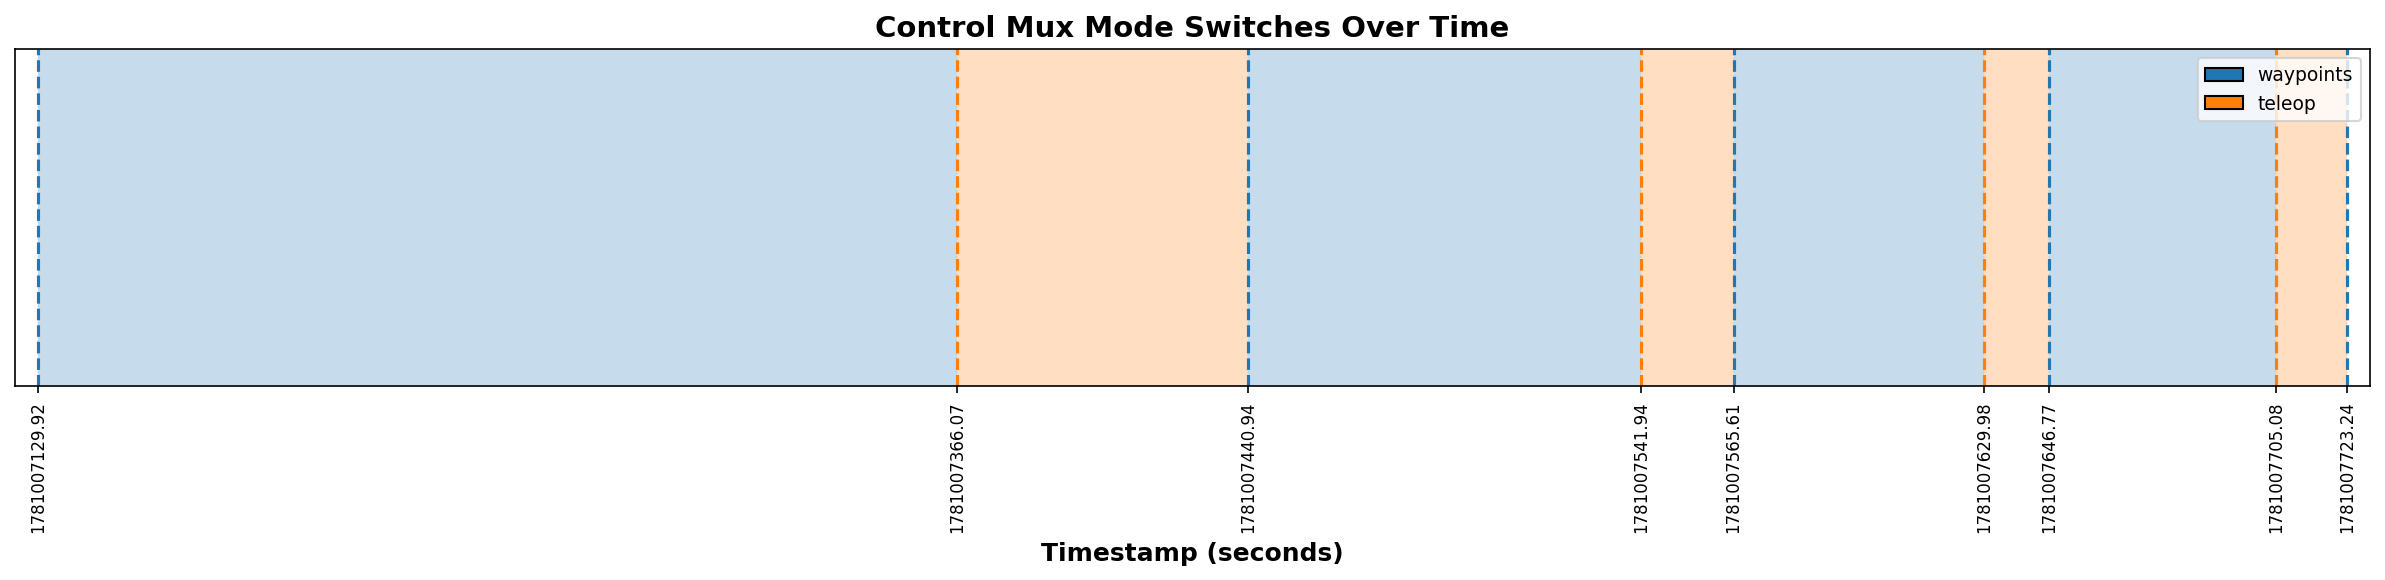
\includegraphics[width=1\linewidth]{Corps_rapport/control_mode_switches.png}
    \captionof{figure}{Timeline des changements de mode de contrôle}
    \label{fig40}
\end{center}

\indent Pour le cas de test illustré en \hyperref[fig40]{Figure 40}, on observe que l'opérateur a repris la main sur le robot en mode téléopération à 4 reprises durant le suivi de waypoints. Cela pourrait traduire une difficulté pour le robot à rallier certains points de passage en toute autonomie.\\

\begin{center}
    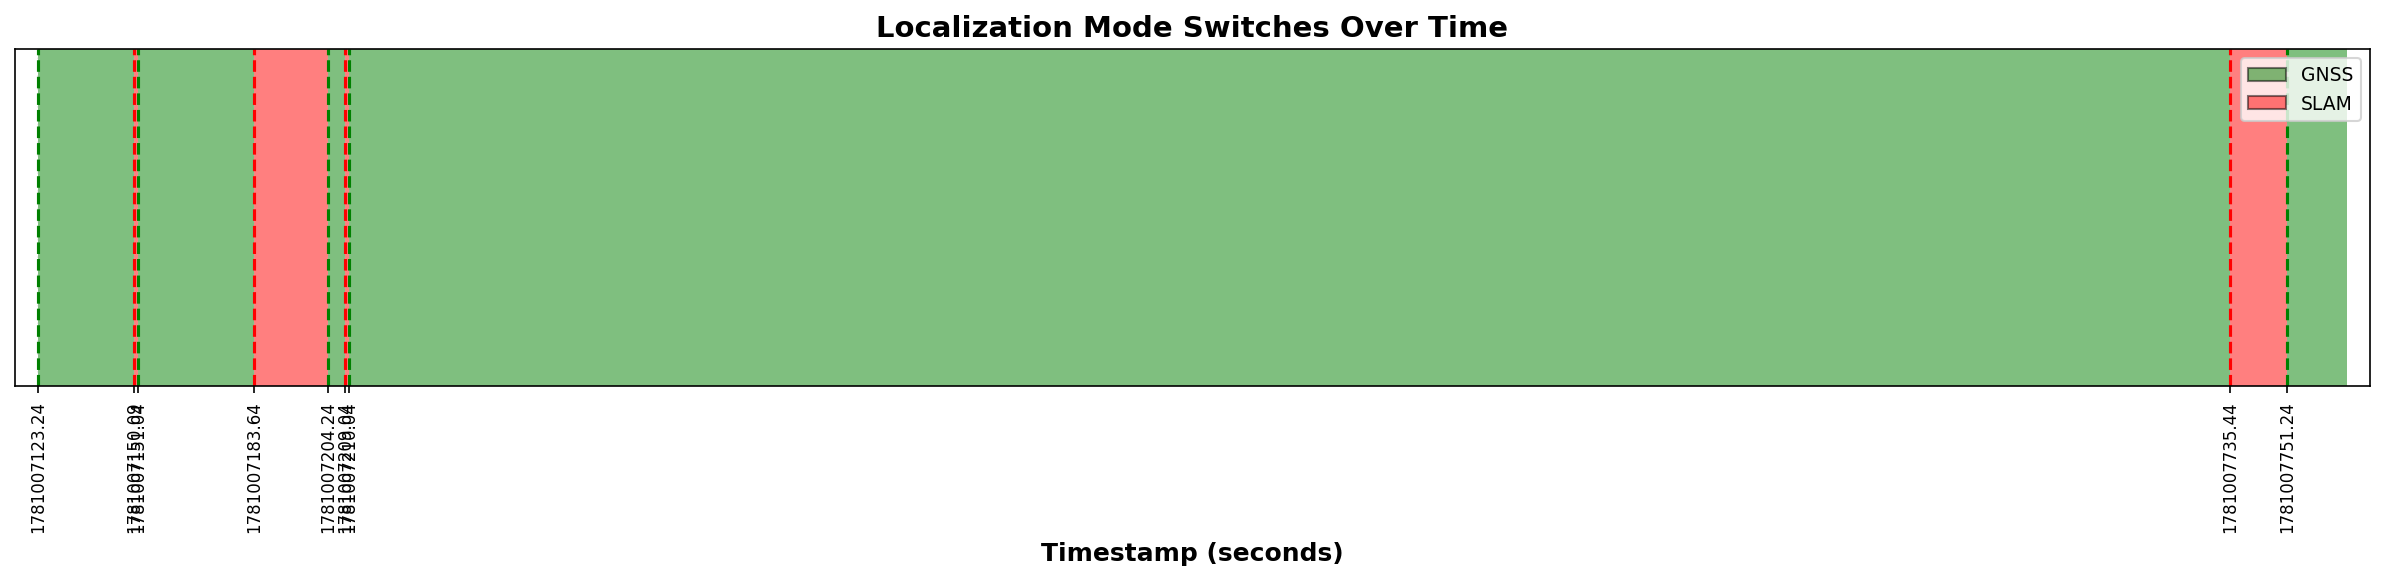
\includegraphics[width=1\linewidth]{Corps_rapport/localization_mode_switches.png}
    \captionof{figure}{Timeline des changements de mode de localisation}
    \label{fig41}
\end{center}

\indent Concernant le cas de test illustré par la \hyperref[fig41]{Figure 41}, on observe que le robot a changé de mode de localisation à 4 reprises durant le suivi de waypoints. Cela pourrait traduire plusieurs passages sous couvert végétal le long du trajet.


\paragraph{Extraction et génération des visualisation de trajectoires et d'erreurs de localisation}

Ce module a pour objectif principal de fournir une représentation visuelle et quantitative des trajectoires du robot (estimées par le SLAM et la centrale inertielle SBG Ellipse) au regard des waypoints (points de passage) à rallier. Afin d'évaluer et de comparer objectivement ces profils de déplacement, la bibliothèque Python EVO a été intégrée à l'architecture de test. L'outil automatisé exploite cette bibliothèque pour générer plusieurs types de livrables graphiques :\\

\begin{itemize}
\renewcommand{\labelitemi}{$\bullet$}
    \item \textbf{Des analyses temporelles} : l'évolution des positions linéaires et angulaires du robot au fil du temps.(\hyperref[fig43]{Figure 43})
    \item \textbf{Des comparaisons spatiales} : la superposition des trajectoires issues du SLAM et de la centrale inertielle SBG.(\hyperref[fig44]{Figure 44})
    \item  \textbf{Des métriques d'erreur} : le calcul et l'affichage de l'erreur de position relative (RPE — Relative Pose Error) pour quantifier la dérive locale du système.\\
\end{itemize}

\indent Afin d'optimiser le traitement, l'architecture de cet outil a été subdivisée en deux modules distincts :\\

\begin{itemize}
\renewcommand{\labelitemi}{$\bullet$}
    \item Le module d'extraction et de sérialisation : Cette première partie est chargée d'extraire les informations pertinentes des topics du fichier bag, puis de les enregistrer dans un fichier CSV. Les données y sont structurées sous forme de tableau indexé par horodatage (timestamp), où chaque colonne correspond à un attribut spécifique et exploitable du message d'origine.
    \item Le module d'analyse et de visualisation : Cette seconde partie assure la lecture du fichier CSV et prend en charge la génération des différentes figures d'analyse.\\
\end{itemize}

\indent Cette conception modulaire et découplée présente un double intérêt opérationnel. D'une part, elle évite de réexécuter la phase d'extraction des données du bag (processus qui peut etre lourd et chronophage) lors d'un simple ajustement graphique ou d'une modification des figures d'analyse. D'autre part, elle permet de générer un fichier CSV intermédiaire. Ce support, considérablement plus léger qu'un fichier bag, assure la persistance de données pré-traitées et exploitables pour des analyses ultérieures.\\

\indent Pour la première partie du traitement, l'outil génère ainsi un fichier CSV indexé par horodatage contenant les colonnes associées aux différents champs des messages pour les topics de type :\\

\begin{itemize}
\renewcommand{\labelitemi}{$\bullet$}
    \item \textbf{geometry\_msgs/TwistStamped} : Champ linéaire et angulaire de la vitesse afin d'avoir les vitesses de consigne envoyées au robot à chaque instant
    \item \textbf{nav\_msgs/Odometry} : Pose du robot dans les différents modes de localisation (SLAM, SBG) pour des tracés de trajectoires.
    \item \textbf{nav\_msgs/Path} : Liste et coordonnées des waypoints à rallier par le robot pour les tracés sur trajectoires.
    \item \textbf{sensor\_msgs/Imu} : Mesures inertielle pour les tracés d'orientation du robot tout au long de la trajectoire.
    \item \textbf{diagnostic\_msgs/DiagnosticArray} : Diagnostics de l'IHM pour l'identification des changements de mode de localisation afin de les superposer sur les tracés de trajectoires.\\ 
\end{itemize} 

\indent Pour la seconde partie du traitement, l'outil exploite les données du CSV pour générer une série de visualisations détaillées, complétée par des métriques d'évaluation standardisées. Ces livrables graphiques se divisent en deux catégories principales :

\subparagraph{a. Les figures d'analyse dynamique et comportementale}:

Ces tracés permettent de caractériser finement le comportement cinématique et l'état du système tout au long de son parcours : \\

\begin{itemize}
\renewcommand{\labelitemi}{$\bullet$}
    \item \textbf{Analyse spatiale et trajectographie} : Superposition et comparaison des trajectoires estimées par le SLAM et par la centrale inertielle (SBG Systems), avec projection des points de passage (waypoints) cibles.
    \item \textbf{Modes de localisation} : Visualisation temporelle et géographique du mode de localisation actif (SLAM ou GNSS RTK) sur les différentes portions de la trajectoire.(\hyperref[fig44]{Figure 44})
    \item \textbf{Attitude du châssis} : Évolution des angles d'orientation de roulis (roll) et de tangage (pitch) du robot le long de la trajectoire, permettant d'identifier d'éventuelles orientations dangereuses liées au relief.
    \item \textbf{Suivi de consigne en vitesse} : Confrontation des vitesses linéaires et angulaires de consigne avec les vitesses réelles mesurées sur le robot.
    \item \textbf{Analyse des écarts de vitesse} : Évaluation des erreurs de vitesse instantanées par rapport aux vitesses de consigne requises pour le ralliement des waypoints.(\hyperref[fig44]{Figure 44})
    \item \textbf{Performances temporelles du suivi} : Mesure fine de la durée de ralliement pour chaque waypoint intermédiaire, ainsi que le calcul du temps total d'exécution de la mission de suivi de trajectoire.
\end{itemize}

\subparagraph{b. Les figures d'évaluation géométrique de la trajectoire}:

En complément de ces analyses comportementales, l'outil intègre un module d'évaluation métrologique s'appuyant sur la bibliothèque EVO. Ce module génère automatiquement des figures d'évaluation standardisées, permettant notamment de quantifier l'erreur de pose absolue (APE - Absolute Pose Error) et l'erreur relative de pose (RPE - Relative Pose Error) par rapport à la trajectoire de référence comme présenté dans la section 2.3.\\

\indent Le processus débute par l'analyse du fichier d'enregistrement (bag file), dont l'objectif est d'extraire et de sauvegarder dans un CSV les valeurs des champs d'un ensemble de topics : \\

\begin{itemize}
\renewcommand{\labelitemi}{$\bullet$}
    \item \textbf{/dlio/dlio\_odom/transformed\_slam\_pose} et \textbf{/sbg/localization} : Pour la localisation SLAM et GNSS du robot.
    \item \textbf{/nav\_stack/function\_waypoints/waypoints\_iterator/path\_in} : Pour l'ensemble des waypoints à rallier par le robot.
    \item \textbf{/barakuda/cmd\_vel} : Pour les commandes / consignes en vitesses envoyées au robot.
    \item \textbf{/main\_odometry} : Pour extraire les vitesses réelles suivies par le robot peu importe le mode de localisation.
    \item \textbf{/nav\_stack/function\_waypoints/waypoints\_iterator/next\_waypoint\_speed} : Pour extraire les vitesses de consigne souhaitées par le robot pour le ralliement des waypoints.
    \item \textbf{/sherpa\_board/xsens\_mti/imu} : Pour extraire les angles d'orientation du robot (roulis et tangage) à chaque instant.
    \item \textbf{/diagnostics} : Pour extraire les diagnostics de l'IHM et identifier les changements de mode de localisation.\\
\end{itemize}

Une fois le CSV généré, l'outil exploite ces données pour produire automatiquement des figures resultant de tracé de colonnes vs colonnes ou de colonnes vs timestamps, ainsi que des figures d'évaluation standardisées (APE et RPE) à l'aide de la bibliothèque EVO. Ces visualisations permettent d'obtenir une vue d'ensemble du comportement du robot, de ses performances de localisation et de son suivi de trajectoire, facilitant ainsi l'identification des anomalies et l'optimisation des algorithmes de navigation. La figure (\hyperref[fig42]{Figure 42}) suivante illustre l'organigramme de cet outil:

\begin{center}
    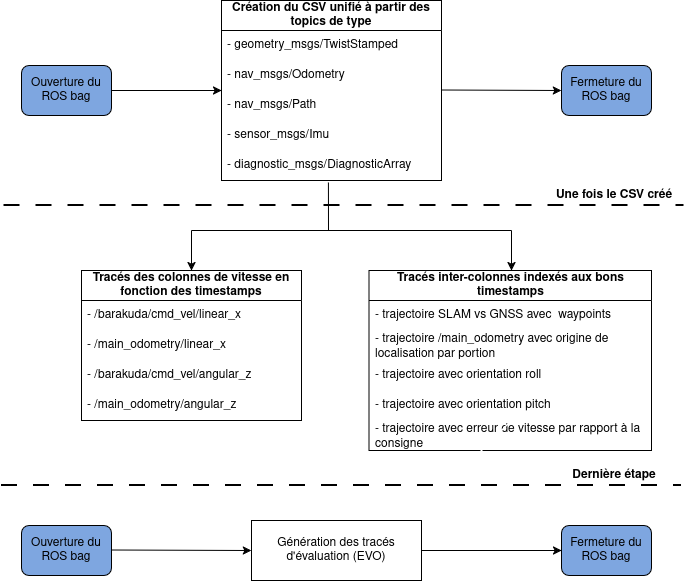
\includegraphics[width=0.7\linewidth]{Corps_rapport/org_viz_extractor.png}
    \captionof{figure}{Organigramme de l'outil d'extraction et de génération des visualisations}
    \label{fig42}
\end{center}
$\ $\

Comme résultat, l'outil génère plusieurs graphiques dont les figures (\hyperref[fig43]{Figure 43} et \hyperref[fig44]{Figure 44}) suivantes :\\

\begin{figure}[H]
    \centering
    \begin{subfigure}[b]{0.46\textwidth}
        \centering
        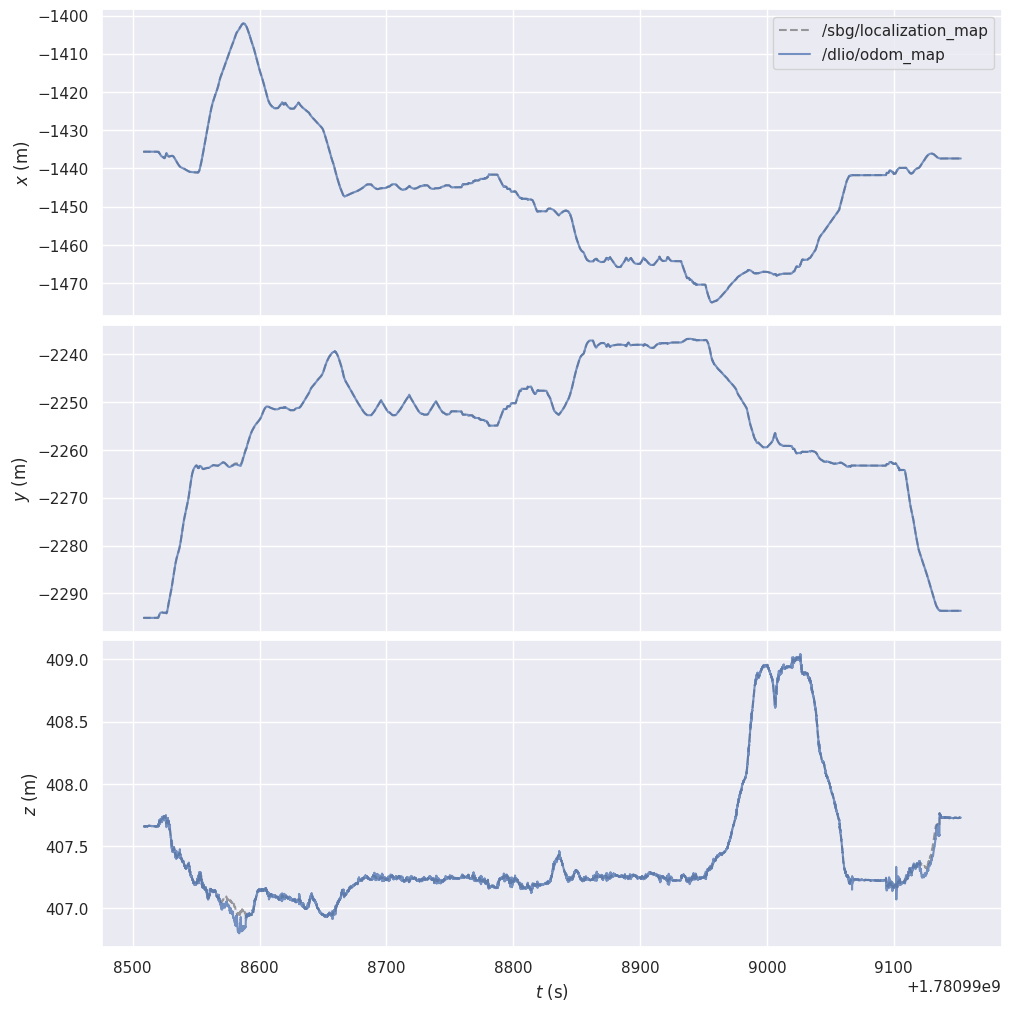
\includegraphics[width=\textwidth]{Corps_rapport/evo_trajectory_analysis_xyz.png}        
    \end{subfigure}
    \hfill
    \begin{subfigure}[b]{0.46\textwidth}
        \centering
        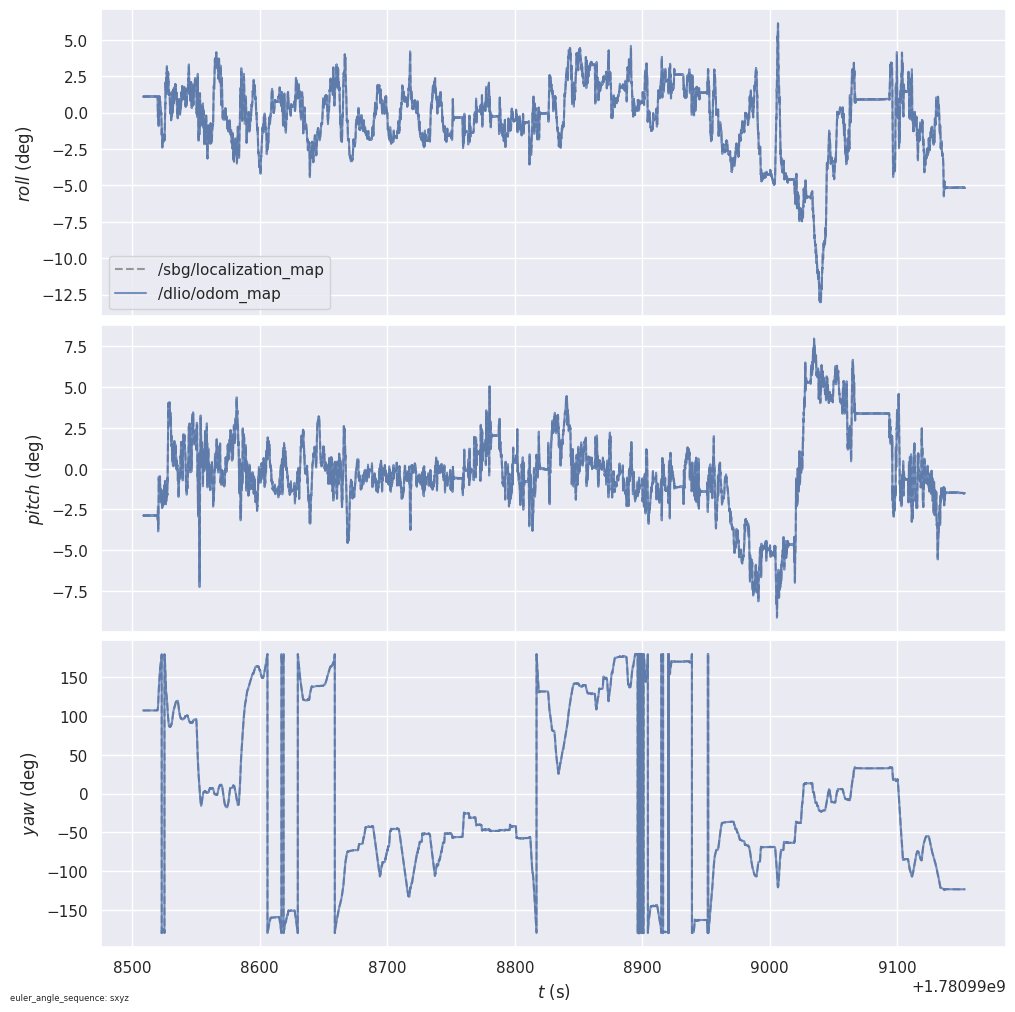
\includegraphics[width=\textwidth]{Corps_rapport/evo_trajectory_analysis_rpy.png}
    \end{subfigure}
    \caption{Visualisation et comparaison des positions linéaires et angulaires du robot}
    \label{fig43}
\end{figure}

\indent La figure \hyperref[fig43]{Figure 43} illustre la très bonne estimation de la pose du robot par le SLAM DLIO par rapport à la vérité terrain fournie par la centrale SBG. On observe que les positions linéaires et les orientations angulaires estimées par le SLAM sont très proches de celles mesurées par la centrale inertielle, ce qui confirme la précision et la fiabilité du SLAM DLIO pour la navigation.

\begin{figure}[H]
    \centering
    \begin{subfigure}[b]{0.46\textwidth}
        \centering
        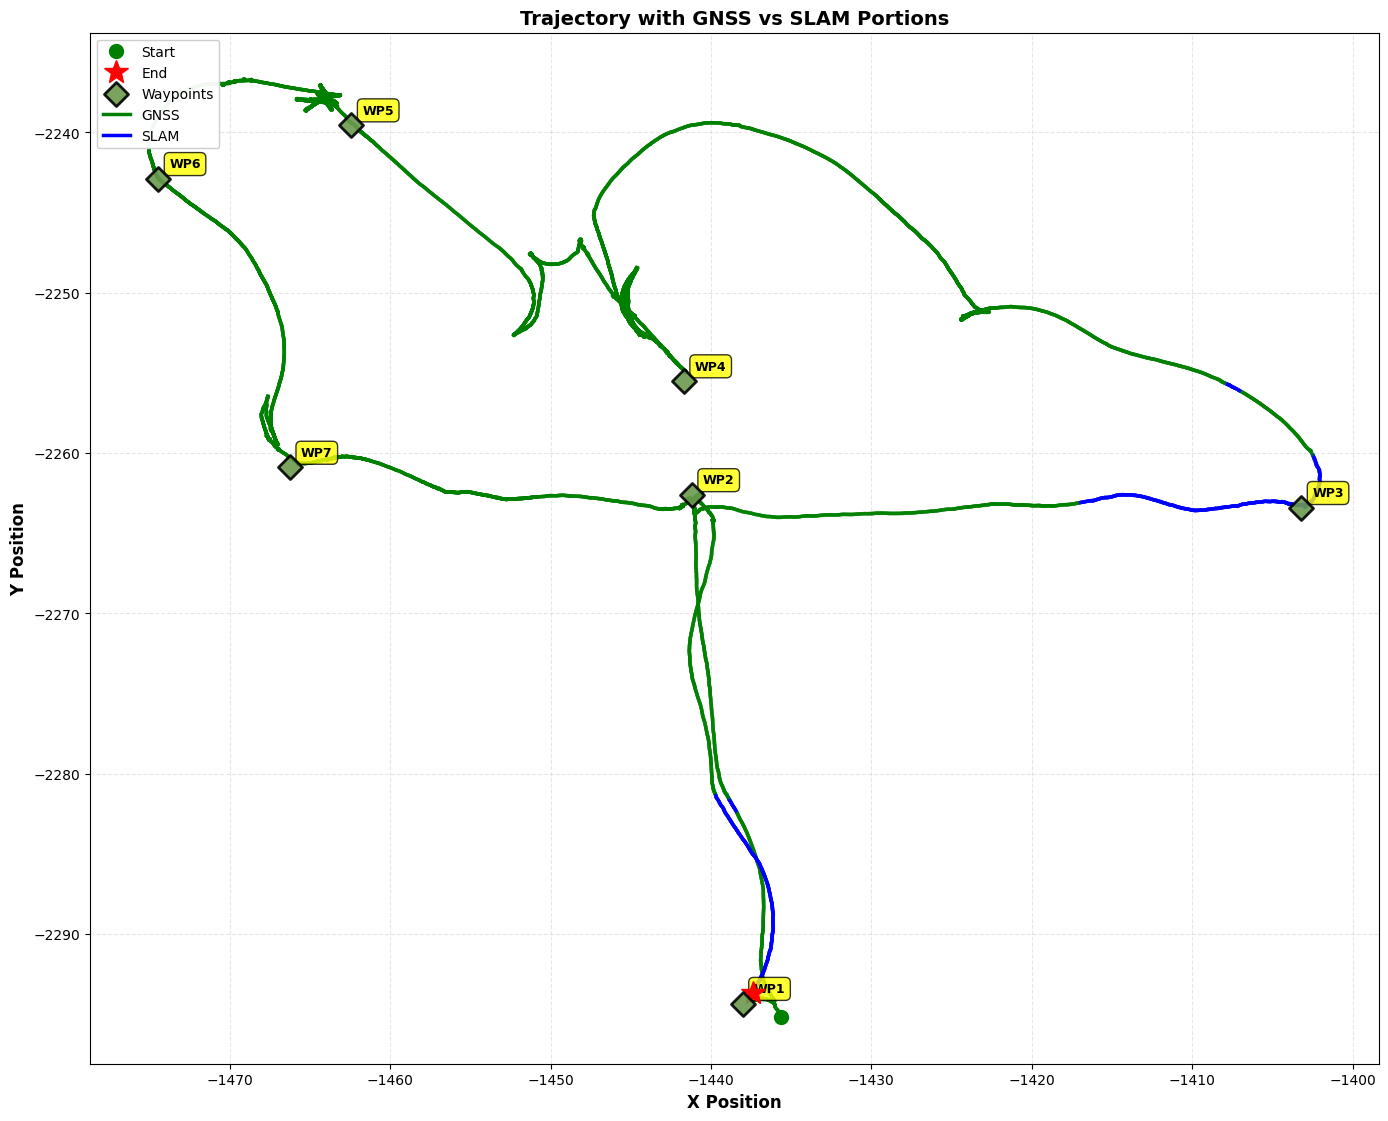
\includegraphics[width=\textwidth]{Corps_rapport/trajectory_gnss_vs_slam.png}        
    \end{subfigure}
    \hfill
    \begin{subfigure}[b]{0.5\textwidth}
        \centering
        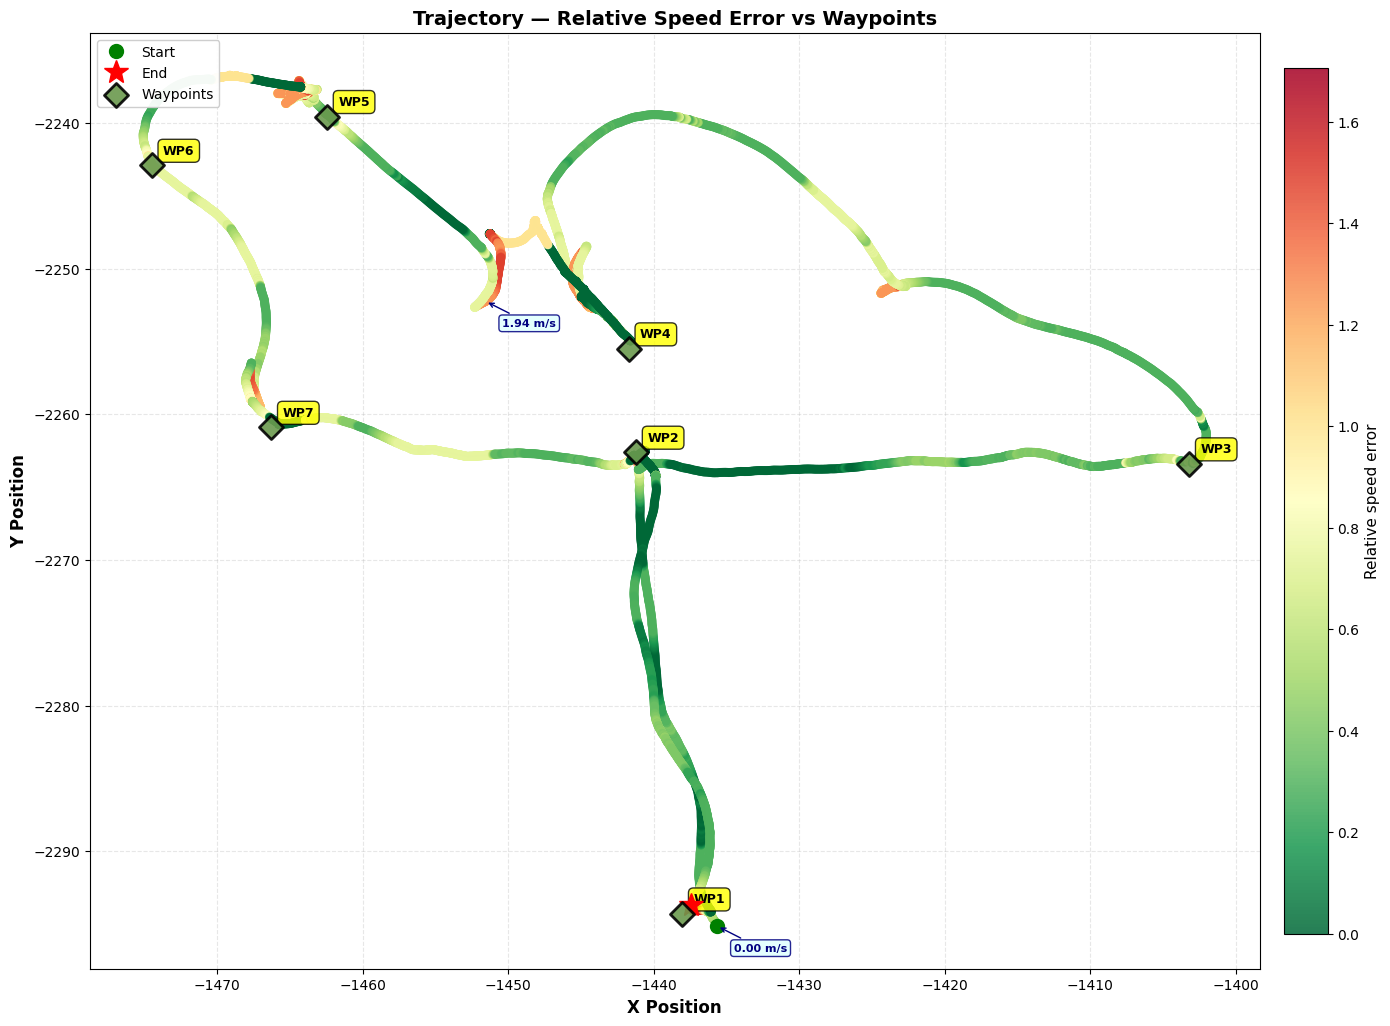
\includegraphics[width=\textwidth]{Corps_rapport/trajectory_speed_error.png}
    \end{subfigure}
    \caption{Evaluation des portions GNSS et SLAM de la trajectoire et erreur de vitesse le long de la trajectoire}
    \label{fig44}
\end{figure}
 
\indent La figure \hyperref[fig44]{Figure 44} met en évidence les portions de la trajectoire où le SLAM DLIO a été utilisé pour la localisation, ainsi que celles où le GNSS RTK a été employé. Elle pourra être comparée à la carte de végétation du site afin de vérifier que les zones de basculement automatique vers le SLAM correspondent effectivement aux zones de couvert. De plus, cette figure illustre les écarts de vitesse le long du parcours, permettant d'identifier les zones de fort ralentissement.\\

\indent Ces visualisations synthétiques permettent d'identifier rapidement les écarts géométriques entre les différentes méthodes de localisation et d'analyser finement les performances de la brique de navigation selon les scénarios de test. Il convient toutefois de souligner que la pertinence de ces indicateurs de performance (KPI) reste conditionnée à la validité de la vérité terrain (ground truth). Celle-ci nécessite une continuité absolue des données de positionnement, ce qui implique l'absence de masquage ou de perte du signal GNSS RTK durant l'acquisition des données.\\


\paragraph{Extraction et génération des vidéos de l'évolution des cartes et du retour vidéo sur l'IHM}

Ce module a pour objectif principal de fournir une représentation visuelle dynamique (vidéo) de l'évolution du MNE (Modèle Numérique d'Élévation), de la planification globale et locale, ainsi que du retour vidéo affiché sur l'interface homme-machine (IHM). S'il n'est pas spécifié de topic particulier en paramètre, l'outil automatise l'extraction des données de l'ensemble des topics \textbf{sensor\_msgs/Image} et \textbf{sensor\_msgs/CompressedImage} présents dans le rosbag. Après décodage des trames, une vidéo synchronisée est générée pour chaque topic au moyen de la bibliothèque OpenCV. Les différents topics d'images ne publiant pas à la même fréquence, l'outil effectue un rééchantillonnage temporel basé sur le timestamp des messages. Un pas temporel commun est calculé en se basant sur le topic possédant la fréquence d'échantillonnage la plus basse. Ainsi, selon leur fréquence d'origine, certains topics ne conservent qu'une image sur deux, voire une image sur quatre pour l'assemblage de leur vidéo respective. Afin d'aligner le début et la fin de l'ensemble des vidéos générées, un offset temporel est appliqué. Ce timestamp d'origine est déterminé par le topic d'image dont la première publication est la plus tardive ; toutes les trames antérieures à cet offset sont ignorées. L'outil génère ainsi un ensemble de vidéos parfaitement synchronisées. Enfin, ces flux sont unifiés au sein d'une vidéo composite par un assemblage image par image (frame-by-frame).  La figure (\hyperref[fig45]{Figure 45}) suivante illustre l'organigramme de cet outil:\\

\begin{center}
    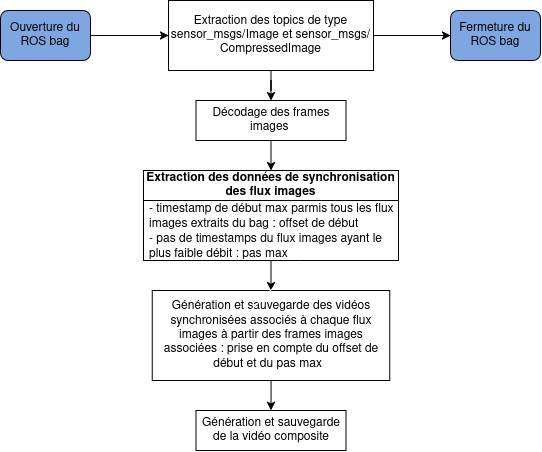
\includegraphics[width=0.7\linewidth]{Corps_rapport/org_video_extractor.png}
    \captionof{figure}{Organigramme de l'outil d'extraction et de génération de vidéos}
    \label{fig45}
\end{center}

\indent La figure (\hyperref[fig46]{Figure 46}) suivante illustre un exemple de vidéo composite générée par l'outil, montrant l'évolution des cartes et du retour vidéo sur l'IHM. Cette vidéo composite offre ainsi une vue d'ensemble du comportement du système durant les essais et permet d'observer, dans l'ordre de lecture (de gauche à droite et de haut en bas) :\\

\begin{itemize}
\renewcommand{\labelitemi}{$\bullet$}
    \item la planification globale de trajectoire. 
    \item la planification locale de trajectoire. 
    \item la carte des gradients d'élévation autour du robot. 
    \item le MNE (Modèle Numérique d'Élévation). 
    \item la visualisation LiDAR.
    \item la vue annotée de l'IHM. \\
\end{itemize}

\begin{center}
    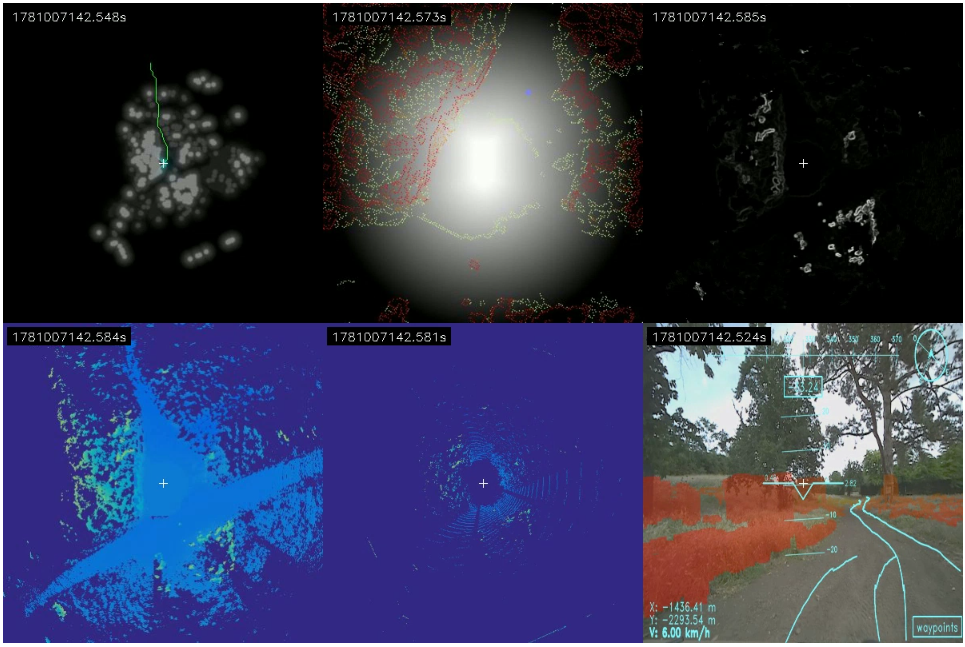
\includegraphics[width=0.7\linewidth]{Corps_rapport/video_aggra.png}
    \captionof{figure}{Vidéo composite des différentes cartes et du retour vidéo sur l'IHM}
    \label{fig46}
\end{center}


\paragraph{Structuration modulaire du générateur de rapports}

\indent Une fois le générateur de rapports de test rendu fonctionnel, l'objectif suivant a consisté à lui apporter une structure modulaire. Cette modularité devait permettre à l'utilisateur de sélectionner à la carte les informations à intégrer dans le rapport final, parmi les options suivantes : diagnostics, visualisation de trajectoires et vidéos. Pour ce faire, j'ai suivi les recommandations d'un ingénieur de l'équipe et me suis tourné vers les bibliothèques Rich et Typer. Rich permet d'améliorer l'affichage dans le terminal, rendant l'expérience utilisateur plus attrayante, tandis que Typer facilite la création d'applications en ligne de commande avec la possibilité de passer des arguments pour spécifier les éléments à générer dans le rapport. L'outil se presente comme le montre la figure suivante (\hyperref[fig47]{Figure 47}):\\
 
\begin{center}
    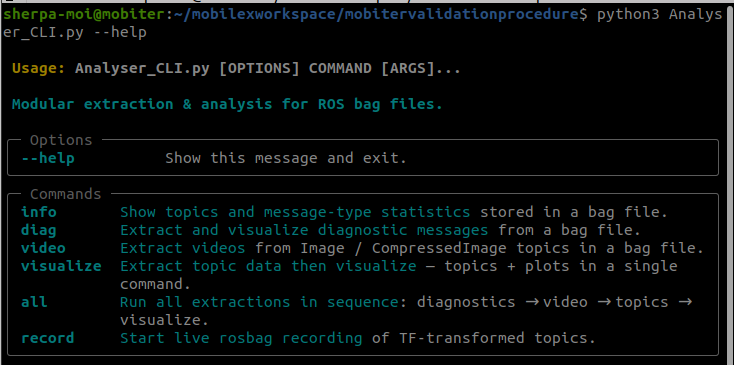
\includegraphics[width=0.7\linewidth]{Corps_rapport/presentation_outil_extraction.png}
    \captionof{figure}{Visualisation terminal de l'outil de génération automatique de rapport de test}
    \label{fig47}
\end{center}


















\subsubsection{Proposition de méthode d'automatisation de la validation de tests en robotique mobile: cas d'application sur Mobiter}

La validation des systèmes autonomes (robots agricoles, drones, véhicules autonomes, robots sous-marins) repose traditionnellement sur des expérimentations sur le terrain. Bien qu'indispensables, ces essais réels présentent de fortes contraintes : un coût financier élevé, des risques matériels et humains, ainsi qu'une répétabilité limitée en raison de la variabilité des conditions environnementales.  

Pour répondre à ces limites, le test en simulation s'est imposé comme une démarche complémentaire majeure. Il permet d'exécuter de façon intensive des suites de tests à moindre coût et en toute sécurité. Les architectures logicielles de simulation se déclinent principalement sous trois formes :  \\

\begin{itemize}
    \item Model-in-the-Loop (MiL) : vérification précoce sur des modèles abstraits (ex. Simulink).
    \item Software-in-the-Loop (SiL) : intégration du logiciel embarqué réel dans un environnement virtuel simulant capteurs et actionneurs.
    \item Hardware-in-the-Loop (HiL) / Vehicle-in-the-Loop (ViL) : exécution sur le matériel physique connecté à des composants virtuels.\\
\end{itemize}

L'automatisation complète de la chaîne de validation soulevait trois verrous scientifiques et techniques fondamentaux : la spécification d'un oracle de test automatisé, la génération de cas de test contraints et variés, et la prise en compte du non-déterminisme.

\paragraph{Méthode basée sur la spécification et l'automatisation des oracles de test}

Le problème de l'oracle de test consiste à déterminer automatiquement si le comportement observé lors d'une exécution correspond au comportement attendu. En robotique autonome, la définition d'un oracle est complexe en raison de l'effet « boule de neige » des décisions logicielles, du volume massif de données produites et de l'absence de spécification complète.

\subparagraph{Oracles basés sur des invariants et propriétés de sûreté}:

Pour contourner la difficulté de prédiction exacte de la trajectoire d'un robot, une approche privilégiée consiste à définir des oracles spécifiés reposant sur des invariants fonctionnels et de sécurité.\cite{2021TOU30119b}  \\

Dans les travaux portant sur le robot agricole Oz et le robot sous-marin REMI, les oracles ont été formalisés autour d'une classification de propriétés :  \\

\begin{itemize}
    \item Propriétés liées aux phases de mission : contrôle du respect de la séquence d'étapes (ex. suivi de ligne, manœuvre de demi-tour, transition vers l'inter-rang suivant).
    \item Seuils physiques et cinématiques : vérification des vitesses maximales, des angles de braquage ou des accélérations par rapport aux limites de sécurité fixées.
    \item Événements catastrophiques et sécurité : détection de collisions, franchissement des limites du terrain, déclenchement inapproprié des arrêts d'urgence ou dépassement des seuils de batterie.
    \item Gestion des erreurs et perception : vérification de la cohérence des messages d'erreur et de la bonne détection des repères visuels ou laser (ex. piquets de fin de rang).  \\
\end{itemize}

Ces oracles peuvent fournir un verdict binaire (Pass/Fail) ou un score quantifié (ex. degré d'écart par rapport à une consigne), permettant de cerner les défaillances par niveau de sévérité.




\subparagraph{Oracles métamorphiques}:

Lorsque la spécification exacte est absente, les oracles peuvent reposer sur des relations métamorphiques. Cela consiste à vérifier la cohérence des sorties entre plusieurs exécutions liées par des transformations géométriques ou environnementales (ex. invariance du comportement sous rotation ou translation du terrain).




\paragraph{Méthodes basées sur la génération automatique de cas de test contraints}

Pour alimenter les campagnes de tests en simulation, il est nécessaire de générer automatiquement des environnements virtuels complexes (topographie, obstacles, conditions de mission).\cite{2021TOU30119b} 

\subparagraph{Approches existantes : Reproduction vs Génération procédurale}:

Reproduction de cas réels : extraction de scènes virtuelles à partir de données réelles enregistrées (cartes GPS, nuages de points). Très utilisée dans l'automobile, cette méthode est limitée par la faible diversité des scènes rejouées. 

Génération procédurale : création synthétique reposant sur des algorithmes stochastiques (ex. bruit de Perlin pour les cartes de hauteur/relief). Elle assure une forte diversité, mais peine à respecter strictement des règles métiers complexes.  

\subparagraph{Approche déclarative hybride : Le framework TAF (Testing Automation Framework)}:

Pour surmonter les limites des approches traditionnelles de type generate-then-filter (inaptes aux environnements très contraints), Clément Robert propose le framework TAF. TAF repose sur un langage spécifique au domaine basé sur XML (XML-TAF) combinant un modèle de données purement déclaratif et la gestion de contraintes complexes.  

L'architecture de TAF met en œuvre une méthode de résolution hybride :\\

\begin{itemize}
    \item Modélisation abstraite : description des entités de la scène (légumes, rangées, obstacles, paramètres de mission) sous forme de nœuds et de paramètres régis par des distributions statistiques.
    \item Résolution par couche et solveur SMT : utilisation d'un solveur SMT (ex. Z3) pour résoudre les contraintes logiques et arithmétiques inter-variables, couplée à un échantillonnage aléatoire pour préserver la diversité des données générées.\\
\end{itemize}

Évalué sur plusieurs cas d'étude (dont la génération de champs de légumes pour le robot Oz), TAF démontre des performances supérieures ou compétitives par rapport à des outils comme PLEDGE, tout en garantissant un haut niveau de couverture de l'espace de test. 


\paragraph{Prise en compte du non-déterminisme et tests de non-régression}

L'application des tests de non-régression en robotique mobile se heurte au non-déterminisme intrinsèque des systèmes autonomes.

\subparagraph{Origines du non-déterminisme}:

Le comportement d'un robot varie entre deux exécutions d'un même cas de test. Ce phénomène découle de plusieurs facteurs :  \\

\begin{itemize}
    \item L'architecture logicielle multithread et les communications asynchrones en best-effort (ex. middlewares comme ROS).
    \item L'utilisation d'algorithmes décisionnels approchés (heuristiques de planification de trajectoire).
    \item Les décalages horlogers et concurrences propres à la plate-forme de simulation elle-même.\\
\end{itemize}

\subparagraph{Stratégie de répétition vs exploration}:

Pour qu'un test de non-régression fournisse un verdict fiable (éviter les faux positifs ou négatifs dûs au non-déterminisme), les travaux de [Robert et al., IRC 2020] préconisent d'évaluer l'impact du nombre de répétitions. En exécutant de façon répétée une suite de tests ($X_{N,M}$ exécutions), l'étude démontre que :  \\

\begin{itemize}
    \item Une exécution unique est insuffisante pour garantir la détection d'une défaillance intermittente.  
    \item Un compromis optimal entre coût de calcul et fiabilité de détection permet de fixer un nombre minimal de répétitions (ex. 5 répétitions par cas de test) pour stabiliser le verdict d'oracle.  
\end{itemize}



\paragraph{Synthèse et perspectives} 

L'automatisation du test en robotique mobile repose sur une chaîne outillée intégrée : \\

\begin{itemize}
    \item Modélisation déclarative et génération SMT (TAF) pour créer des environnements structurés, variés et physiquement valides.
    \item Exécution en simulation SiL (Gazebo/ROS) répétée plusieurs fois pour absorber le non-déterminisme du système.
    \item Analyse automatisée par oracles basés sur des invariants pour porter un verdict binaire ou quantifié sans intervention humaine.\\
\end{itemize}

Ces recherches démontrent que le test en simulation ne doit plus être considéré comme un simple outil de prototypage, mais comme un pilier rigoureux et automatisé du processus de qualification et de non-régression des logiciels autonomes critiques.

















\subsubsection{Robustification du mode suivi de lisière : gestion d'obstacles sur le chemin de suivi}

Comme présenté dans la section 2.2, le mode de suivi de lisière est un mode de navigation autonome conçu pour permettre au robot de longer une lisière d'arbres ou de végétation. Cependant, lors des campagnes de tests, ce mode a révélé des limites opérationnelles majeures en présence d'obstacles non franchissables obstruant le chemin de suivi.\\

\indent En effet, face à un obstacle, le robot s'immobilisait systématiquement. Ce blocage s'explique par le paramétrage de sécurité du planificateur local (local planner) associé à ce mode, configuré pour inhiber les commandes de vitesse générées par le correcteur de pure poursuite (pure pursuit) dès qu'une trajectoire entrait en collision avec un obstacle. Ce comportement passif s'est avéré particulièrement pénalisant et non viable dans le cadre du Défi 3 du challenge.\\

\indent Pour pallier cette faiblesse, une première approche a consisté à optimiser l'algorithme de détection de lisière en élargissant le rayon du cercle d'analyse. L'objectif était d'intégrer les obstacles proches de la lisière (seuil fixé à 1,5 mètre) afin qu'ils soient directement assimilés à la lisière elle-même, forçant ainsi le robot à la contourner naturellement. Néanmoins, cette solution s'est avérée insuffisante pour deux raisons majeures :\\

\begin{itemize}
\renewcommand{\labelitemi}{$\bullet$}
    \item \textbf{Obstacles isolés} : Elle ne permettait pas de traiter les obstacles situés au centre du chemin de suivi, trop éloignés de la lisière pour entrer dans le rayon d'analyse étendu.
    \item \textbf{Perte de référence visuelle (Masquage)} : Lors de l'amorce de la manœuvre d'évitement, la trajectoire d'évitement éloignait le robot de sa trajectoire nominale, lui faisant perdre de vue la lisière de référence qu'il suivait initialement.\\
\end{itemize}

\indent De plus, l'augmentation arbitraire du rayon du cercle de détection a introduit un effet de bord critique. Cette modification réduit en effet l'aptitude du système à détecter la continuité de la lisière située immédiatement derrière l'obstacle (si celui-ci n'est pas très proche de la lisière), créant ainsi une "zone d'ombre" algorithmique, comme l'illustre la figure ci-dessous (\hyperref[fig48]{Figure 48}): \\

\begin{figure}[H]
    \centering
    \begin{subfigure}[b]{0.6\textwidth}
        \centering
        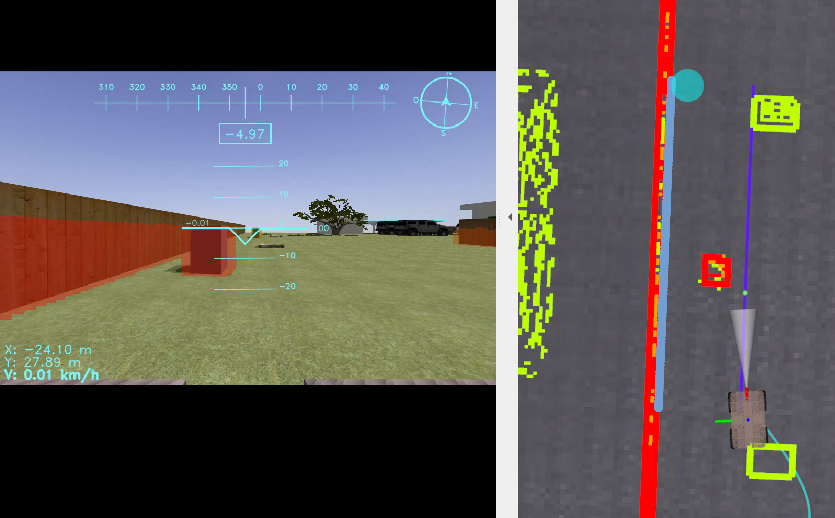
\includegraphics[width=\textwidth]{Corps_rapport/suivi_lisiere_05.png}        
    \end{subfigure}
    \hfill
    \begin{subfigure}[b]{0.25\textwidth}
        \centering
        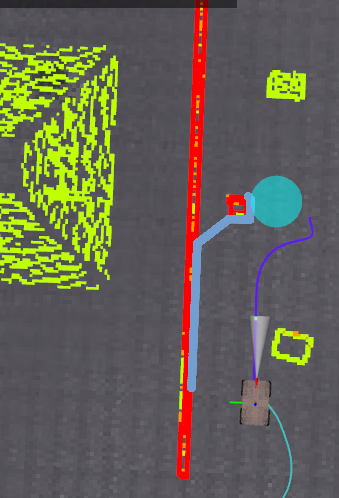
\includegraphics[width=\textwidth]{Corps_rapport/suivi_lisiere_1.png}
    \end{subfigure}
    \caption{Evaluation de la taille du cercle de détection de lisière sur la capacité à détecter la continuité de la lisière derrière un obstacle}
    \label{fig48}
\end{figure}

\indent L'idée suivante était de garder un petit cercle et d'introduire un mécanisme de mise à jour intelligent du chemin de suivi. Au début de mon stage, ce chemin était actualisé à chaque nouvelle détection de lisière, ce qui posait des problèmes lors des manœuvres de contournement d'obstacle car un nouveau chemin était calculé à partir de la lisière détectée sur l'obstacle lors de la manœuvre. L'objectif était donc de mettre à jour le chemin courant si et seulement si le nouveau chemin issu de la nouvelle détection de lisière est cohérent. Par cohérent, nous entendons un test de longueur de chemin car la longueur d'une lisière suivie ne baisse pas drastiquement entre deux déplacements élémentaires successifs du robot.\\

\indent Face aux limites des ajustements purement géométriques, l'approche retenue a consisté à conserver un rayon de détection restreint (garantissant un bon pouvoir de résolution) tout en introduisant un mécanisme de filtrage et de mise à jour dynamique cohérent du chemin de suivi. Initialement, le chemin de référence du robot était recalculé et écrasé de manière asynchrone à chaque nouvelle détection de lisière. Lors des phases de contournement, ce comportement générait des instabilités critiques : l'algorithme interprétait l'obstacle lui-même comme la nouvelle lisière à suivre, perturbant ainsi la trajectoire globale du robot.\\

\indent Pour résoudre ce problème, une logique de transition d'état conditionnelle a été implémentée. Désormais, le chemin courant n'est mis à jour par une nouvelle détection que si cette dernière respecte un critère de cohérence spatio-temporelle. Ce filtre repose sur l'hypothèse physique selon laquelle la longueur d'une lisière continue ne peut subir de variation drastique (diminution brutale) entre deux pas de calcul successifs du système (de l'ordre de quelques millisecondes). Mathématiquement, soit $L_{t}$ la longueur du chemin issu de la détection à l'instant $t$, et $L_{t-1}$ la longueur du chemin précédemment validé. La mise à jour du chemin de navigation est autorisée si et seulement si la longueur du nouveau chemin respecte l'équation suivante \eqref{eq8}:

\begin{equation}
\frac{L_{t-1}}{2} \leq L_{t}
\label{eq8}
\end{equation}

\begin{itemize}
\renewcommand{\labelitemi}{$\bullet$}
    \item \textbf{En cas de détection cohérente} : Si la condition est respectée, le chemin est mis à jour, garantissant l'adaptation du robot aux légères courbures de la lisière.
    \item \textbf{En cas d'anomalie ou de masquage} : Si la condition n'est pas respectée, la mise à jour est inhibée. Le robot conserve et suit son chemin précédent, ce qui lui permet de franchir la zone de perturbation (l'obstacle).\\
\end{itemize}

Malgré plusieurs ajustements fins (\textit{fine-tuning}) des paramètres du planificateur local et du contrôleur \textit{Pure Pursuit} — notamment l'augmentation de l'horizon de planification, la réduction du coût de rotation autour de l'axe $z$ pour le planificateur et l'accroissement de la distance de visée (\textit{lookahead distance}) du contrôleur —, le robot ne parvenait pas à contourner les obstacles présents sur la trajectoire de suivi. Il a été conclu que le contrôleur \textit{Pure Pursuit} n'offrait pas une liberté suffisante au planificateur local de type DWA (\textit{Dynamic Window Approach}). Ce dernier, agissant dans l'espace des commandes, ne pouvait pas modifier suffisamment les consignes de vitesse pour écarter le robot des obstacles. Une solution efficace consistait donc à déformer le chemin généré par l'algorithme de détection de lisière en amont du contrôleur \textit{Pure Pursuit}.\\

À cette fin, nous avons choisi d'implémenter un premier planificateur local dans l'espace de la tâche. Ce module prend en entrée le chemin issu de la détection de lisière ainsi que le nuage de points obstacles au tour du robot. Il génère une nouvelle trajectoire qui garantit le suivi de la lisière à la distance souhaitée tout en évitant les obstacles. Ce nouveau chemin est ensuite transmis au contrôleur \textit{Pure Pursuit}, dont les commandes de vitesse (linéaire et angulaire) sont vérifiées puis ajustées, si nécessaire, par le second planificateur local de type DWA avant d'être envoyées au robot.(\hyperref[fig49]{Figure 49})\\

Après concertation avec mon tuteur et d'autres membres de l'équipe, l'algorithme \textit{Elastic Band} (bandes élastiques) \cite{eband} a été choisi pour réaliser ce planificateur dans l'espace de la tâche.\\

\begin{center}
    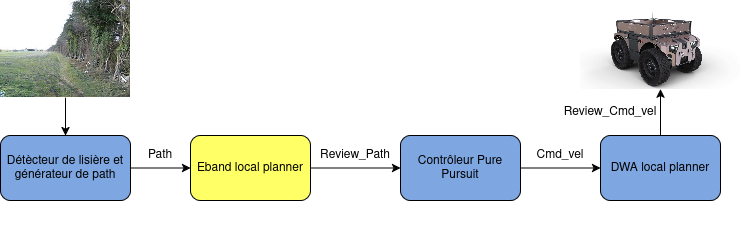
\includegraphics[width=1.0\linewidth]{Corps_rapport/org_review_border_follow.png}
    \captionof{figure}{Flowchart du mode de suivi de lisière revu}
    \label{fig49}
\end{center}

Dans la figure ci-dessus, sont représentés en bleu les modules déjà existants dans la stack MOBITER et en jaune le module à rajouter.

\paragraph{Fonctionnement du planificateur Elastic Band}

L'approche par \textbf{bandes élastiques} articule la planification globale et le contrôle réactif en temps réel en modélisant une trajectoire initiale sans collision sous la forme d'une structure flexible soumise à des forces virtuelles. En s'ajustant dynamiquement aux flux de données capteurs, la bande se déforme pour générer un parcours fluide et sécurisé face aux obstacles fixes ou mobiles, tout en minimisant localement sa longueur et en conservant la topologie du chemin d'origine. L'intérêt majeur de cette méthode réside dans son optimisation incrémentale : la qualité de la trajectoire s'affine continuellement à mesure que le robot progresse, tout en maintenant une charge de calcul minimale à chaque itération.\\

L’approche des bandes élastiques telle que proposée à l'origine se compose principalement de deux étapes : 

\begin{itemize}
\renewcommand{\labelitemi}{$\bullet$}
    \item \textbf{raffinement de la bande} : Cette étape consiste à supprimer les bulles inutiles et à combler les lacunes de la bande afin de réduire la charge de calcul.
    \item \textbf{optimisation de la bande} : Cette étape consiste à calculer les forces internes et externes et à modifier les positions des bulles en conséquence.
\end{itemize}


\subparagraph{a. Le concept des Bulles (Bubbles)}:

Pour fonctionner à des fréquences compatibles avec le contrôle temps réel ($\approx 10\text{ Hz}$ à $100\text{ Hz}$), l'algorithme évite le calcul coûteux de l'espace de configuration libre ($C\text{-space}$) global. Il introduit la notion de bulle de liberté locale $B(b)$.\\

\begin{itemize}

    \item \textbf{Définition géométrique (cas holonome 2D)} : Pour une configuration $b$, si $p(b)$ représente la distance minimale absolue entre le robot et l'obstacle le plus proche, la bulle $B(b)$ est définie par le disque centré sur $b$ et de rayon $q$ tel que:
    
    \begin{equation}
        B(b) = \{q : \Vert{}b - q\Vert{} < p(b)\}  
        \label{eq9}
    \end{equation}

    Tout point situé à l'intérieur de cette bulle garantit l'absence de collision avec l'environnement. \\

    \item \textbf{Extension aux robots orientables (3 DDL : $x, y, \theta$)} : La métrique de distance intègre la rotation via le rayon maximal $r_{\max}$ de la géométrie du robot par rapport à son centre :
    
    \begin{equation}
        D(\Delta b) = \sqrt{\Delta b_x^2 + \Delta b_y^2} + r_{\max} \vert{}\Delta b_\theta\vert{}
        \label{eq10}
    \end{equation}

    La bulle 3D s'exprime alors comme $B(b) = \{q : D(b - q) < p(b)\}$. \\

    \item \textbf{Condition de continuité de la bande} : La bande élastique est constituée d'une chaîne discrète de postures (via-points) associées à leurs bulles respectives. Pour garantir l'existence d'une trajectoire continue sans collision, deux bulles consécutives $B(b_i)$ et $B(b_{i+1})$ doivent obligatoirement se chevaucher ($\text{Overlap} \neq \emptyset$).\\

    \item \textbf{Adaptabilité spatiale} : La densité de discrétisation varie automatiquement. En zone dégagée, les bulles sont grandes et espacées, tandis qu'à proximité des obstacles, les bulles rétrécissent, augmentant la résolution locale du chemin.

\end{itemize}


\subparagraph{b. Modélisation de la déformation par forces artificielles}:

La forme du chemin est régie par un système de forces artificielles appliquées à chaque bulle $b_i$, cherchant un état d'équilibre quasi-statique. \\

\begin{itemize}

    \item \textbf{Force totale ($f$)} : La force totale appliquée à la bulle $b_i$ est la somme vectorielle des forces internes de contraction et des forces externes de répulsion :
    
    \begin{equation}
        f = f_c + f_r
        \label{eq11}
    \end{equation}

    \item \textbf{Force interne de contraction ($f_c$)} : Elle simule la tension mécanique d'un élastique pour raccourcir le chemin et supprimer le mou (slack) provoqué par les contours inutiles :
    
    \begin{equation}
        f_c = k_c \left( \frac{b_{i-1} - b_i}{\Vert{}b_{i-1} - b_i\Vert{}} + \frac{b_{i+1} - b_i}{\Vert{}b_{i+1} - b_i\Vert{}} \right)
        \label{eq12}
    \end{equation}

    où $k_c$ est le gain de tension interne. Les forces sont normalisées pour maintenir une tension uniforme le long de la chaîne. \\

    \item \textbf{Force externe de répulsion ($f_r$)} : Elle repousse la bande hors des zones à haut risque pour maximiser la marge de sécurité autour des obstacles :
    
    \begin{equation}
        f_r = \begin{cases}  k_r (\rho_0 - p) \dfrac{\partial p}{\partial b} & \text{si } p < \rho_0 \\  0 & \text{si } p \ge \rho_0  \end{cases}
        \label{eq13}
    \end{equation}    
    
    où $k_r$ est le gain de répulsion et $\rho_0$ représente le rayon d'influence de l'obstacle. Le gradient $\frac{\partial p}{\partial b}$ est estimé par différences finies locales. \\

    \item \textbf{Force modifiée et stabilité ($f^*$)} : Afin d'éviter le glissement longitudinal indésirable des bulles le long de la bande (ce qui provoquerait des cycles infinis de création/suppression de points), la force totale subie par une bulle est projetée sur l'axe orthogonal à la trajectoire :
    
    \begin{equation}
        f^* = f - \frac{f \cdot (b_{i-1} - b_{i+1})}{\Vert{}b_{i-1} - b_{i+1}\Vert{}^2} (b_{i-1} - b_{i+1})
        \label{eq14}
    \end{equation}

\end{itemize}

Lors du déplacement du robot ou des obstacles, la bande ajuste sa structure topologique par ré-échantillonnage :  \\
\begin{itemize}
\renewcommand{\labelitemi}{$\rightarrow$}
    \item Insertion de bulles : Si l'écartement entre deux bulles adjacentes devient trop grand au point de rompre leur chevauchement, une nouvelle bulle est insérée au milieu pour restaurer l'intégrité topologique du chemin. Si l'insertion échoue à rétablir le recouvrement, le déplacement est invalidé (signal d'échec nécessitant une re-planification globale).  
    \item Suppression de bulles : Si la bulle $B(b_i)$ devient redondante (i.e. si ses deux voisines $B(b_{i-1})$ et $B(b_{i+1})$ se chevauchent directement), la bulle $B(b_i)$ est supprimée pour alléger la charge de calcul.\\
\end{itemize}

 
\begin{comment}
Garantit la continuité $C^1$ de la trajectoire (ex. via splines sous contrainte de bulles), éliminant les arrêts aux angles morts. 
Calcul local basé uniquement sur la distance à l'obstacle le plus proche $p(b)$, dispensant de construire la map $C\text{-space}$ globale.  
Absorbe les bruits de perception et les obstacles imprévus en déformant la trajectoire sans recalculer un plan complet.  
La chaîne de bulles fournit une preuve géométrique formelle que la trajectoire déformée reste strictement sans collision.
\end{comment}

La trajectoire locale modifiée qui en résulte est ensuite transmise à un suiveur de trajectoire local qui calcule le point d’intersection entre la séquence de lignes reliant les centres des bulles et la circonférence de la bulle autour du robot. Le suiveur de trajectoire fait varier la vitesse en fonction de la taille des bulles et calcule enfin une vitesse sûre en tenant compte des limites de vitesse du robot et des bulles suivantes.


\paragraph{Résultats de l'implémentateur de  l'Elastic Band sur le mode de suivi de lisière}

Une fois le rajout de l'algorithme de bandes élastiques implémenté \cite{eband_planner} dans la stack, la modification du chemin de suivi de lisière a été testée en simulation. Les résultats ont montré que le robot était désormais capable de contourner les obstacles présents sur la trajectoire de suivi à condition que ces obstacles ne se trouvent pas directement sur le chemin de suivi car ceci résulte en un échec de l'optimiseur de l'algorithme de bandes élastiques qui se retrouve coincé dans un minimum local. La \hyperref[fig50]{Figure 50} suivante illustre bien cet echec : \\

\begin{figure}[H]
    \centering
    \begin{subfigure}[b]{0.325\textwidth}
        \centering
        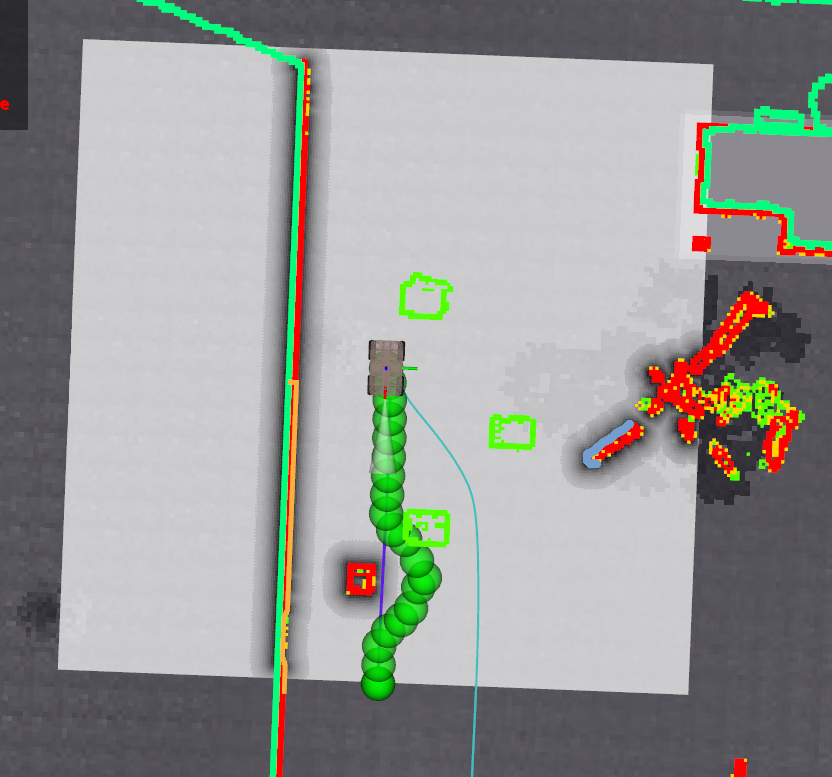
\includegraphics[width=\textwidth]{Corps_rapport/eband_3.png}   
        \caption{Contournement réussi d'un obstacle proche du chemin de suivi sans compression des bulles}
        \label{fig:image1}
    \end{subfigure}
    \hfill
    \begin{subfigure}[b]{0.325\textwidth}
        \centering
        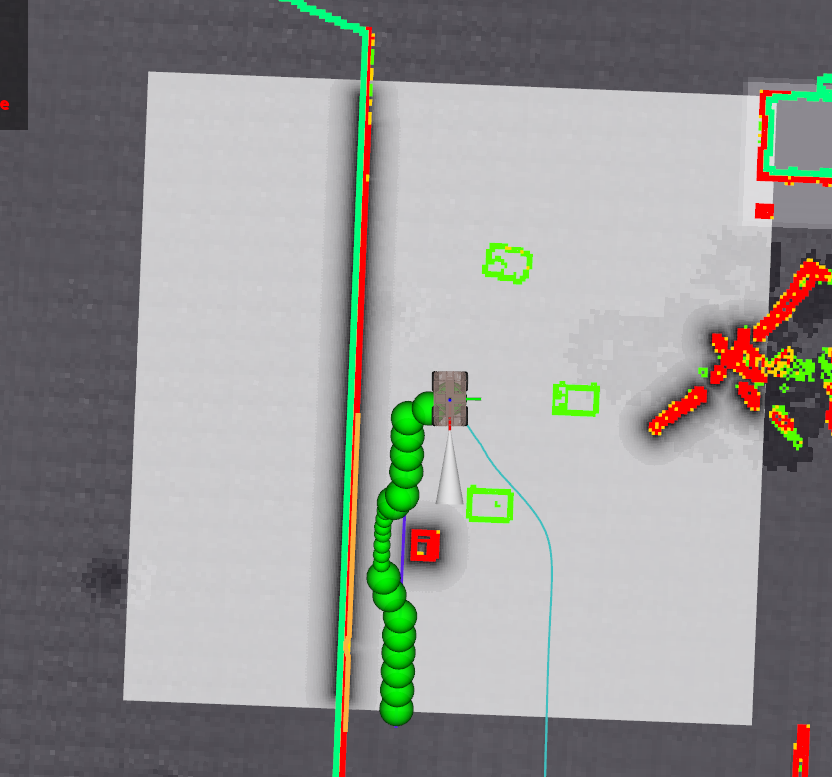
\includegraphics[width=\textwidth]{Corps_rapport/eband_2.png}
        \caption{Contournement réussi d'un obstacle proche du chemin de suivi avec compression des bulles}
        \label{fig:image2}
    \end{subfigure}
    \hfill
    \begin{subfigure}[b]{0.325\textwidth}
        \centering
        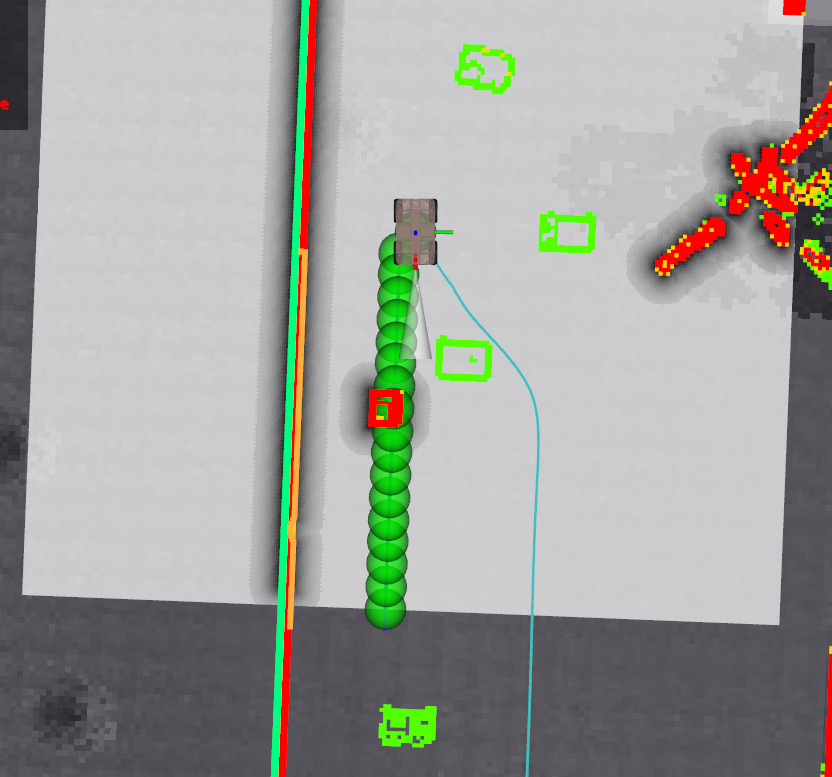
\includegraphics[width=\textwidth]{Corps_rapport/eband_1.png}
        \caption{Échec du contournement d'un obstacle placé directement sur le chemin de suivi}
        \label{fig:image3}
    \end{subfigure}
    \caption{Résultats de l'implémentation de l'algorithme original de bandes élastiques sur le suivi de lisière}
    \label{fig50}
\end{figure}

La \hyperref[fig:image3]{Figure 50(c)} illustre un échec de contournement lorsque l'obstacle est placé directement sur le chemin de suivi. Ce ci est logique car l'optimiseur de l'algorithme de bandes élastiques se retrouve coincé dans un minimum local. En effet, d'apres l'equation \eqref{eq13}, la gradient $\frac{\partial p}{\partial b}$ est nul lorsque le point representatif du robot se trouve sur l'obstacle et $p$ devient nulle, ce qui empêche l'optimiseur de se déplacer vers une position plus sûre car aucune force répulsive n'est générée.\\

La \hyperref[fig:image3]{Figure 50(c)} illustre un échec de contournement lorsque l'obstacle est placé directement sur le chemin de suivi. Ce comportement s'explique par le fait que l'optimiseur de l'algorithme des bandes élastiques se retrouve coincé dans un minimum local. En effet, d'après l'équation \eqref{eq13}, le gradient $\frac{\partial p}{\partial b}$ s'annule lorsque le point représentatif du robot se situe exactement sur l'obstacle et que la distance $p$ devient nulle. Cela empêche l'optimiseur de dévier la trajectoire vers une position plus sûre, aucune force répulsive n'étant alors générée.\\



\paragraph{Modification de l'optimiseur de l'algorithme de bandes élastiques}





















\begin{comment}

\subsubsection{Intégration des dernières modifications de la brique de cartographie après refactoring}
Une fois le projet bien pris en main, une première mission m'a été confiée pour, d'une part, me familiariser avec la méthodologie de versionnement sur Git et, d'autre part, prendre en main la procédure de mise en route du robot et de la Brique MOBILEX*.\\\\
Le projet venait de subir une refonte complète et la brique de cartographie, qui avait été modifiée sur l'ancienne version afin d'ajouter un filtre de Kalman* permettant de pondérer la mise à jour de la carte en fonction de la confiance accordée aux données provenant des capteurs, devait être intégrée à la nouvelle version de la Brique MOBILEX* puis testée. Cette intégration consistait à revoir le mapping des topics et le nom des paquets appelés, ainsi qu'à ajouter l'installation des nouvelles librairies dans la procédure d'installation du projet et leur appel dans les paquets en modifiant les fichiers CMakeLists utilisés pour la compilation* de ces derniers.\\\\
Après avoir intégré et testé en simulation le bon fonctionnement de cette dernière, M. Barbier et moi sommes allés la tester à l'INRAE. Le robot n'ayant pas été réutilisé depuis la refonte du projet, il a fallu, dans un premier temps, remettre l'installation au propre. J'ai ensuite pu me familiariser avec la procédure de mise en route du projet sur le robot.\\\\
Pour tester la brique, nous avons lancé la Brique MOBILEX* complète incluant cette dernière dans des conditions idéales, c'est-à-dire avec une position précise au centimètre fournie par le GNSS RTK. Pour obtenir cette précision, une base fixe dont la position est connue de manière précise compare la position calculée à partir du signal GPS avec sa vraie position et envoie des corrections au récepteur présent sur le robot. Il a alors suffi de couper l'envoi des corrections pour dégrader volontairement la précision de la position afin de s'assurer que la carte ne se dégrade pas trop rapidement.\\\\
Les résultats ont montré que la carte se mettait moins à jour, ce que nous souhaitions, mais que les mesures imprécises restaient tout de même trop prises en compte, rendant la carte inexploitable au bout de quelques secondes (\hyperref[fig20]{Figure 20} et \hyperref[fig21]{21}).\\
\begin{center}
    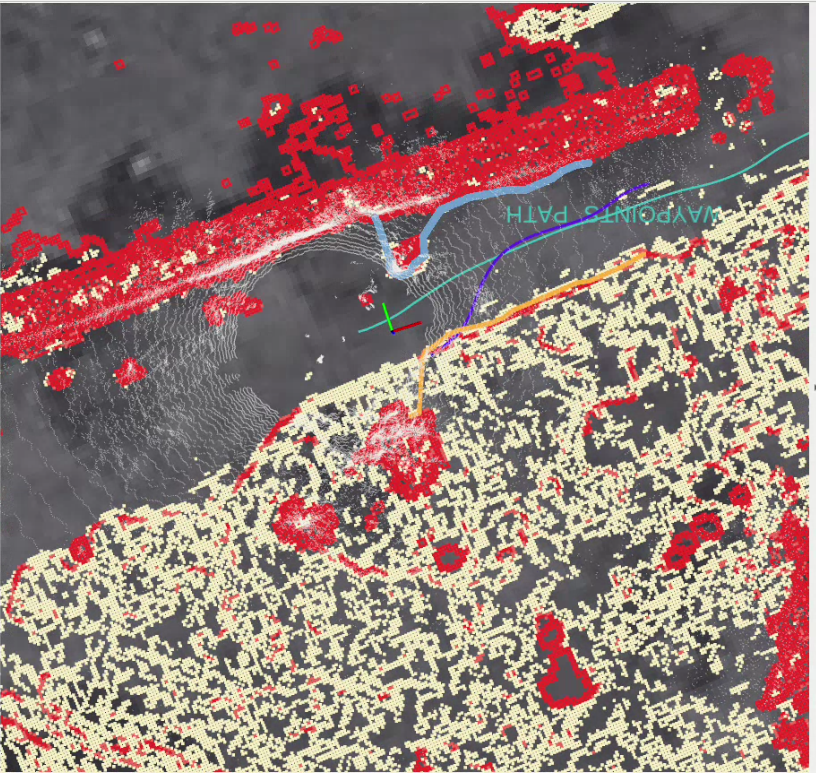
\includegraphics[width=0.7\linewidth]{Corps_rapport/map_rtk.png}
    \captionof{figure}{Carte des obstacles avec GNSS RTK}
    \label{fig20}
\end{center}
\begin{center}
    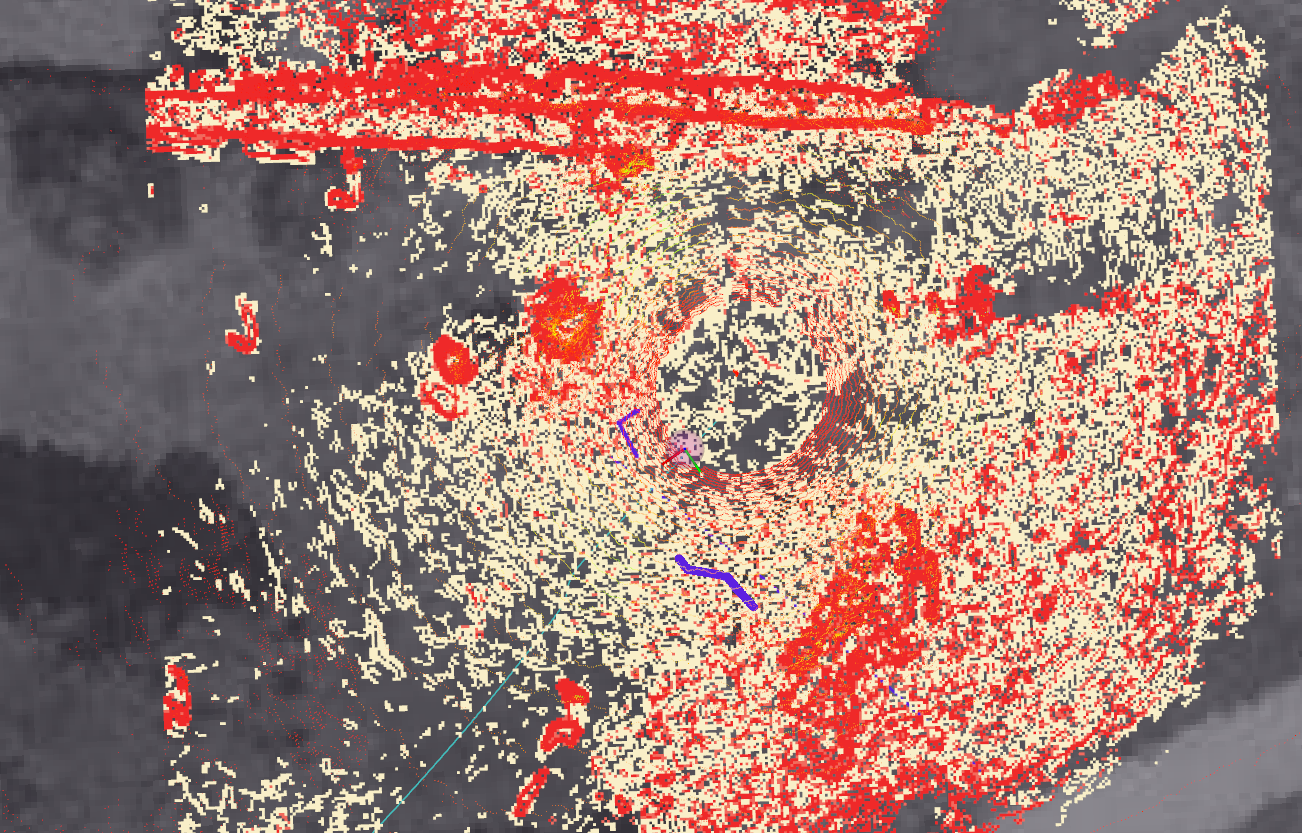
\includegraphics[width=1\linewidth]{Corps_rapport/map_sans_rtk.png}
    \captionof{figure}{Carte des obstacles après 5 secondes de perte des corrections du mode RTK}
    \label{fig21}
\end{center}

Une solution simple a alors été envisagée. Elle consiste à détecter toute anomalie sur le fonctionnement du GNSS en mode RTK pour ajouter un switch visant à sous-estimer la précision de la position retournée dès lors que la fiabilité de la mesure n'est plus garantie (problème de capteur, d'envoi des corrections, de couverture GPS, etc.).\\\\
Pour préparer l'ajout de ce switch, il m'a été demandé d'ajouter une fonction Python permettant de vérifier tout un ensemble de paramètres à tout instant et de publier le résultat de la vérification sous la forme d'un flag.
\subsubsection{Investigations sur un problème de téléopération}
Lors des tests à l'INRAE, la présence d'une personne de l'institut est obligatoire et un ingénieur a été recruté l'an dernier pour encadrer ces tests.\\\\
Lors des tests de la nouvelle brique de cartographie, cette personne a constaté que le robot mettait plus de temps à réagir en téléopération à plus de $2\ m.s^{-1}$ qu'avant le refactoring, que lors de tests réalisés par l'INRAE avec leur propre brique de commande ou qu'en le contrôlant avec la télécommande fournie par SHARK Robotics.\\\\
La téléopération assistée devait être présentée à la DGA lors de la revue d'avancement prévue le mois suivant. M. Barbier et moi avons alors investigué sur ce problème en urgence.\\\\
La première piste explorée fut un délai potentiel au sein de la chaîne de commande. En remontant l'ensemble de la chaîne de commande, nous n'avons pas trouvé de délai entre la réalisation d'une commande à la manette et sa traduction en vitesses de roues à envoyer au robot. Cependant, en comparant les instants d'envois des commandes au robot et le moment où le robot réagissait à ces dernières, on observait un décalage de l'ordre de $0,5\ s$.\\\\
L'hypothèse alors formulée était que notre interface du robot programmée en Python faisait appel à des fonctions de communication provoquant ce délai de $0,5$ seconde, là où l'INRAE utilisait une interface en C++ faisant appel à d'autres fonctions pour communiquer avec le robot ne provoquant pas ce délai. Le problème était que les tests réalisés par l'INRAE remontaient à longtemps et qu'ils n'arrivaient pas à remettre en route leurs codes, mais nous ont dit que leur interface était une adaptation de notre interface pour l'intégrer à leur environnement.\\\\
Nous avons alors décidé de récupérer leur interface pour pouvoir la comparer avec la nôtre et l'intégrer dans notre Brique MOBILEX* pour avoir une interface en C++. Cette réintégration n'a rien changé sur le comportement du robot.\\\\
En examinant la réponse du robot à l'envoi d'une commande en téléopération, je me suis rendu compte qu'en plus du délai de $0,5$ seconde observé, il y avait des dépassements de l'ordre de 30 \% sur la vitesse angulaire, pouvant causer ces difficultés de contrôle.\\\\
J'ai alors proposé de refaire le paramétrage du correcteur de taux de lacet.\\\\
N'ayant pas de modèle du système, nous avons réalisé ce paramétrage à la main comme il est courant de faire pour un correcteur PID. Pour éviter de trop abîmer le terrain, nous avons utilisé des consignes échelons faibles de $0,25\ rad.s^{-1}$.\\\\
En vérifiant le bon fonctionnement du correcteur lors d'un suivi de waypoints, nous nous sommes rendu compte que le modèle que nous cherchions à asservir n'est pas linéaire car là où il n'y avait aucune anomalie notable à $0,25\ rad.s^{-1}$, on observait des dépassements de 20 \% à $2\ rad.s^{-1}$.\\\\
Il a alors été proposé de réaliser une linéarisation par partie du correcteur pour atténuer ces phénomènes, mais que cette solution serait étudiée ultérieurement car elle n'interviendrait pas dans l'urgence actuelle de résoudre les problèmes de téléopération avant la revue d'avancement prévue deux semaines plus tard.\\\\
En inspectant les commandes angulaires fournies par le nœud Joy\_node, nous nous sommes rendu compte que le joystick analogique avait une grande zone morte, faisant passer le joystick de la position nulle à maximale au plus petit mouvement. De plus, les échelles de consignes de vitesse angulaires étaient de $0$ à $3\ rad.s^{-1}$ là où l'INRAE allait de $0$ à $1\ rad.s^{-1}$. L'achat d'un joystick de meilleure qualité et la modification de l'échelle ont permis de grandement améliorer le contrôle du robot lors de virages, mais il restait lent à s'arrêter en comparaison avec le contrôle à la manette fournie par SHARK Robotics.\\\\
La configuration des pentes d'accélération et de décélération dans l'interface du Barakuda a alors été remise en question car l'ancien ingénieur de SHERPA Engineering qui avait travaillé sur l'interface n'avait pas documenté le choix de la limite d'accélération à $1.38\ m.s^{-2}$. Il se trouve que cette valeur avait été donnée à l'oral par un ingénieur de SHARK Robotics pour protéger les variateurs du robot. Cependant, en mesurant les accélérations réalisées par la télécommande du robot, on s'est rendu compte que les limites d'accélérations utilisées sont supérieures à $2.5\ m.s^{-2}$ et que la décélération est encore plus franche car le robot serre ses freins lors du relâchement du joystick.\\\\
Lors d'une réunion organisée par la DGA regroupant l'ensemble des consortiums et des représentants de SHARK Robotics, nous avons posé la question de la nécessité de limiter l'accélération du robot à $1.38\ m.s^{-2}$ alors que la télécommande fournie ne l'est pas, et il se trouve qu'aucun autre consortium n'avait reçu cette indication et les représentants de SHARK Robotics n'étaient pas non plus au courant de cette limitation. Nous avons alors décidé d'aligner nos rampes d'accélérations sur celles de la télécommande du robot, soit $2.5\ m.s^{-2}$, ce qui a résolu le problème de contrôle en téléopération et permis au passage de diminuer le temps de prédiction des LUTs de la planification locale, la rendant plus permissive.
\subsubsection{Installation et test de la sémantique caméra}
Une fois l'urgence résolue, nous avons pu reprendre les tests des ajouts pour le défi 2. Un des grands enjeux du défi 2 à traiter est la présence d'herbes hautes, de fumée et de brouillard parasitant le LIDAR*. \\\\
La solution imaginée pour répondre à cette problématique est l'utilisation de la sémantique caméra.\\\\
La brique de sémantique caméra a alors été développée pour évaluer dans un premier temps la faisabilité de la solution.\\\\
M. Barbier et moi nous sommes alors occupés d'installer l'ensemble des outils utilisés par cette nouvelle brique sur le robot et avons évalué ses performances lors de la détection du sol et de la fumée.\\\\
L'évaluation des performances consistait à vérifier la qualité de la détection du sol, y compris dans les herbes hautes, et de la fumée lorsque le robot est à l'extérieur et à l'intérieur de cette dernière, le tout en s'assurant que la charge CPU et GPU induite par la segmentation* ne compromette pas les performances temps-réel de la Brique MOBILEX*.\\\\
Les résultats obtenus montrent que la segmentation* fonctionne globalement bien pour la détection du sol (\hyperref[fig22]{Figure 22}) malgré certaines frames où le détecteur open-set ne détecte rien, et que les performances temps-réel sont toujours assurées (temps d'inférence* ~60 ms). Cependant, la détection de la fumée n'est quant à elle pas exploitable en l'état. Lorsque le robot est à l'extérieur de la fumée, il ne détecte qu'une partie de cette dernière (\hyperref[fig23]{Figure 23}) et lorsqu'il se situe dans la fumée, le détecteur open-set ne détecte plus rien (\hyperref[fig24]{Figure 24}).\\
\begin{center}
    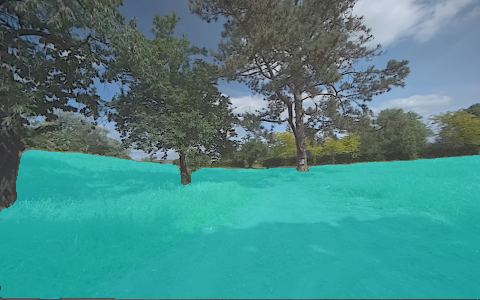
\includegraphics[width=0.8\linewidth]{Corps_rapport/ground.png}
    \captionof{figure}{Segmentation du sol}
    \label{fig22}
\end{center}
\begin{center}
    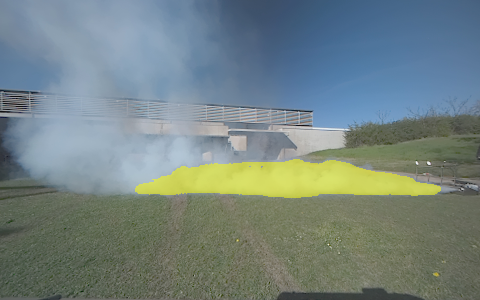
\includegraphics[width=0.8\linewidth]{Corps_rapport/fumee_exterieur.png}
    \captionof{figure}{Segmentation de la fumée depuis l'extérieur}
    \label{fig23}
\end{center}
\begin{center}
    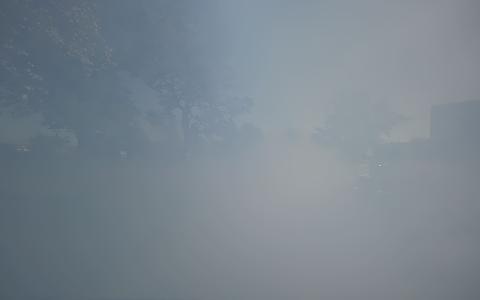
\includegraphics[width=0.8\linewidth]{Corps_rapport/fumee.png}
    \captionof{figure}{Segmentation de la fumée au sein de cette dernière}
    \label{fig24}
\end{center}
\subsubsection{Calibration extrinsèque caméra-LIDAR}
La phase d'évaluation étant concluante pour la détection du sol, l'utilisation de la sémantique caméra a été retenue pour pouvoir naviguer dans les hautes herbes.\\\\
Pour pouvoir intégrer cette solution au projet, il a été nécessaire de réaliser la calibration extrinsèque entre la caméra et le LIDAR*, car ces derniers seront voués à être fusionnés lors de la création de la carte. Plus précisément, la solution planifiée serait de se servir du nuage de points produit par la ZED pour d'une part avoir une redondance capteur pour diminuer le manque d'information dans la carte à l'avant du véhicule et anticiper la gestion des pannes capteurs et d'autre part, fournir une information sémantique dans les différentes tuiles de la carte.\\\\
Étant devenu familier avec la procédure d'utilisation du robot, cette tâche m'a été confiée en toute autonomie.\\\\
La première idée de calibration était de réaliser la calibration à tâtons en projetant le nuage de points LIDAR* dans l'image caméra et de modifier la transformation entre la caméra et le LIDAR* jusqu'à ce que les points se superposent correctement dans une scène contenant des objets de différentes tailles à différentes distances.\\\\
Lors des tests de visualisation de la superposition du nuage de points de la caméra avec celui du LIDAR*, les résultats n'étaient pas concluants, ce qui nous a laissé penser que la calibration réalisée n'était pas suffisamment précise.\\\\
Une calibration plus qualitative a alors été imaginée en réalisant une méthode ICP point-to-plane entre le nuage de points de la caméra et le nuage de points LIDAR*. La méthode ICP point-to-plane est une technique utilisée pour aligner deux nuages de points en trois dimensions. Contrairement à la méthode ICP point-to-point, qui minimise la distance entre les points correspondants des deux nuages, la méthode point-to-plane minimise la distance entre les points d'un nuage et les plans tangents estimés à partir de l'autre nuage de points.\\\\
Cette méthode est souvent préférée dans les applications où les nuages de points ont des densités différentes ou lorsque l'on souhaite obtenir une meilleure précision dans l'alignement, ce qui est notre cas, car le nuage de points de la caméra est bien plus dense que celui du LIDAR*.\\\\
Pour réaliser cette méthode ICP, j'ai commencé par créer un nœud ROS* me permettant d'extraire les nuages de points caméra et LIDAR* dans leur repère respectif et de les enregistrer dans des fichiers binaires. Ensuite, j'ai créé un script Python me permettant de lire le contenu de ses fichiers, de filtrer les points et, en me servant de la bibliothèque Open3D, de réaliser la méthode ICP en point à plan et de visualiser le résultat.\\\\
La calibration par la méthode ICP était sensiblement proche de la précédente et lors de la visualisation avec Open3D (\hyperref[fig25]{Figure 25}) les nuages de points se superposaient bien tandis que lors des tests, la visualisation sur RVIZ était toujours décalée (\hyperref[fig26]{Figure 26}).\\
\newpage
\begin{figure}[h]
    \centering
    \begin{subfigure}[b]{0.7\textwidth}
        \centering
        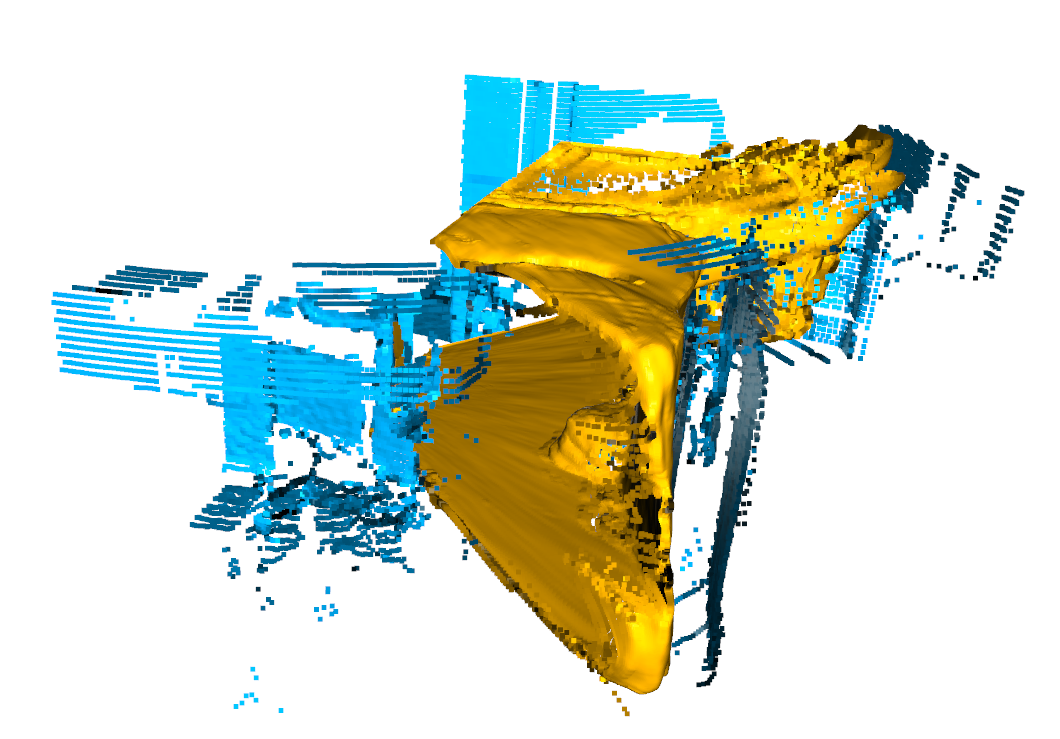
\includegraphics[width=\textwidth]{Corps_rapport/ICP_avant_tf.png}
        \caption{Avant transformation}
        \label{fig:image5}
    \end{subfigure}
    \begin{subfigure}[b]{0.7\textwidth}
        \centering
        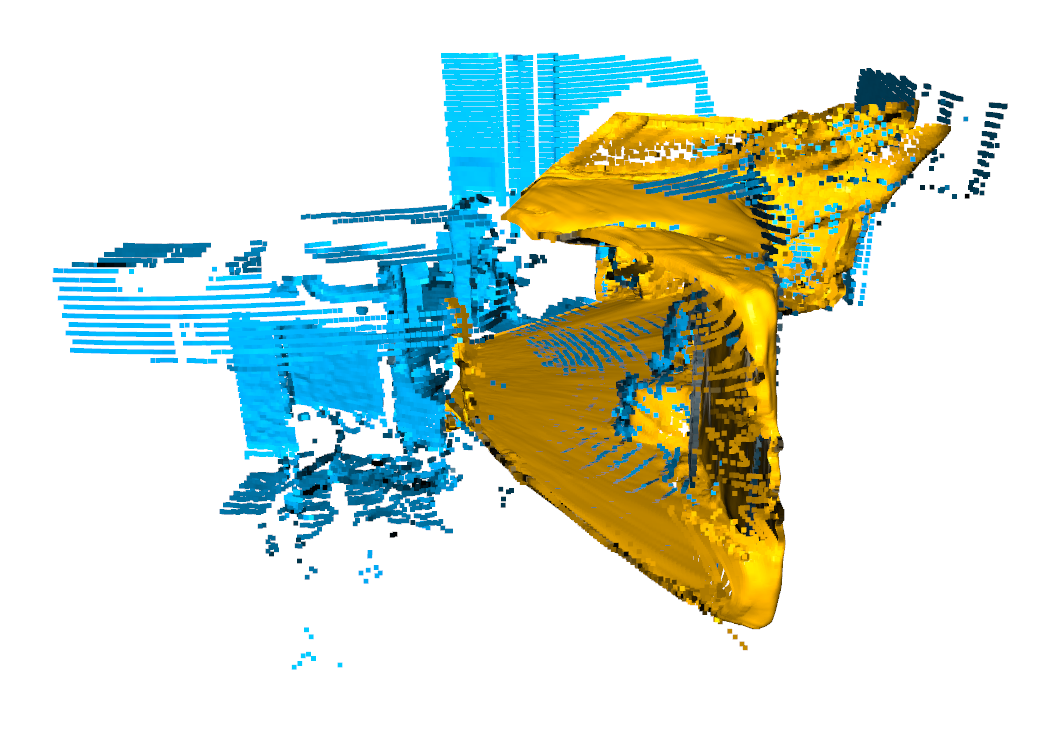
\includegraphics[width=\textwidth]{Corps_rapport/ICP_apres_tf.png}
        \caption{Après transformation}
        \label{fig:image6}
    \end{subfigure}
    \caption{Calibration extrinsèque Caméra-LIDAR par la méthode ICP point to plane}
    \label{fig25}
\end{figure}
\newpage
\begin{center}
    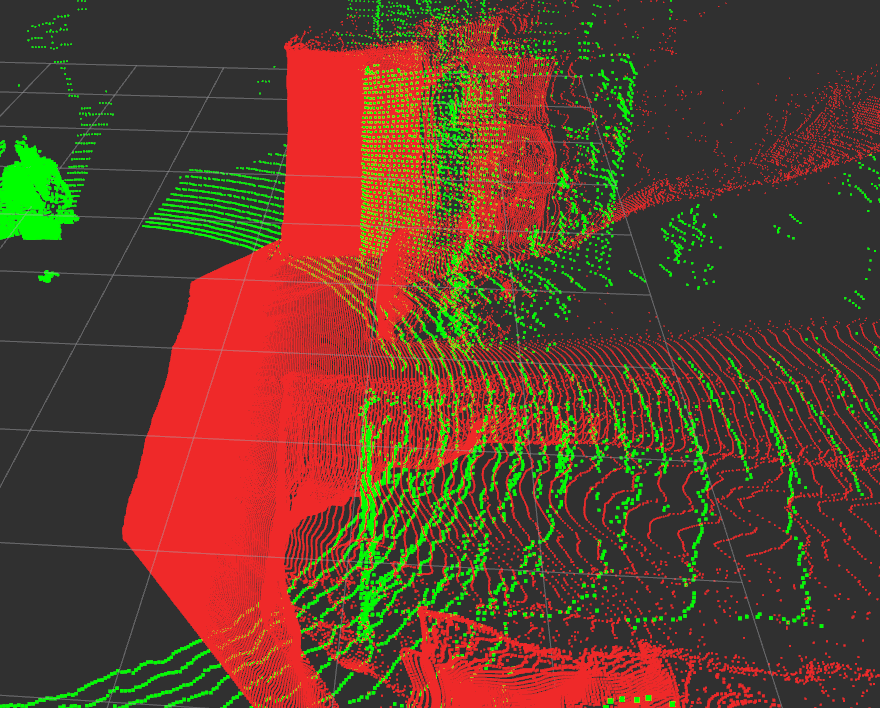
\includegraphics[width= 0.6\linewidth]{Corps_rapport/lidar_camera_mv_tf.png}
    \captionof{figure}{Visualisation de la calibration extrinsèque sous RVIZ}
    \label{fig26}
\end{center}
$\ $\\
Mes doutes se sont alors penchés sur une mauvaise publication de la transformation entre la caméra et le LIDAR* et après un peu d'inspection, je me suis rendu compte que le problème provenait du driver de la caméra qui écrasait continuellement notre transformation en la remplaçant par une transformation identité.\\\\
Après modification du fichier launch du driver, les nuages de points caméra et LIDAR* se superposent comme souhaité (\hyperref[fig27]{Figure 27}).\\
\begin{center}
    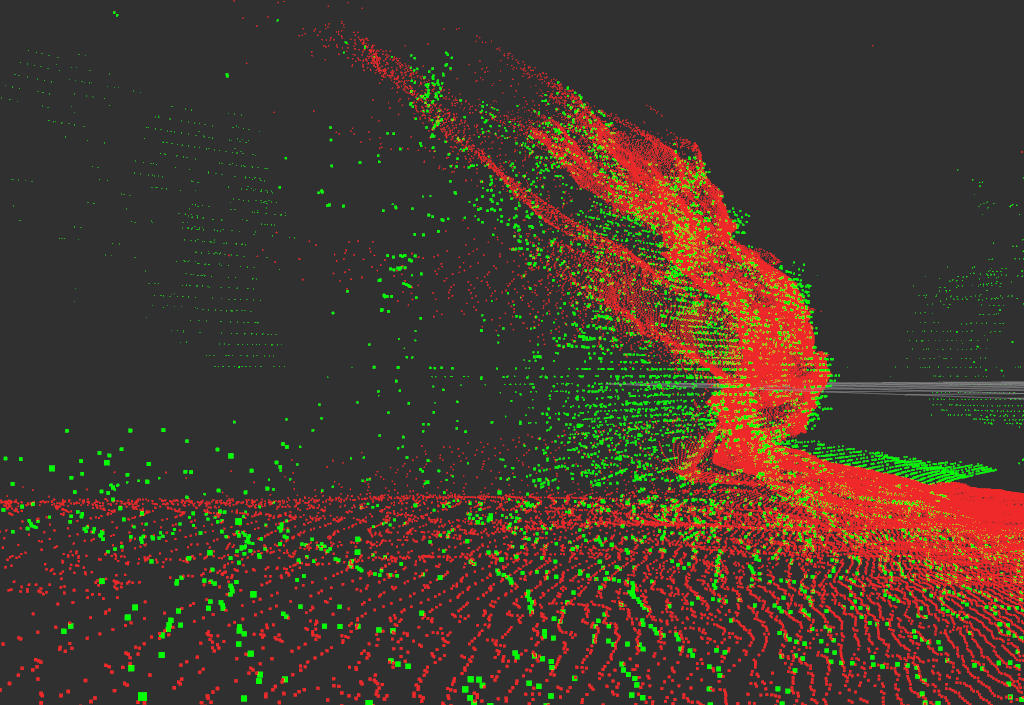
\includegraphics[width=0.8\linewidth]{Corps_rapport/lidar_camera1.png}
    \captionof{figure}{Visualisation de la calibration extrinsèque sous RVIZ après correction du driver}
    \label{fig27}
\end{center}
\subsubsection{Test du nouveau suivi de lisière}
Lors du premier défi, deux problèmes avaient été identifiés : un problème de détection de la lisière lors de la présence d'angles droits et un problème concernant la génération de la trajectoire du suivi de lisière avait été constaté. La trajectoire générée pouvait traverser le bas-côté à suivre. Ce problème était cependant masqué par la couche du local planner qui empêchait au robot d'entrer dans le bas-côté, ce qui faisait que le robot arrivait tout de même à suivre les lisières, mais anormalement lentement.\\\\
Cette génération de trajectoire a alors été modifiée en une translation de la lisière détectée selon la direction de la moyenne des normales de la détection tandis que le problème de détection dans les angles droits a été rectifié en ajustant les paramètres du détecteur.\\\\
Lors de mes tests de ces modifications, je me suis rendu compte que la lisière fluctuait d'une détection à l'autre, ce qui forçait le correcteur à diminuer sa vitesse pour tenter de s'aligner en permanence à la trajectoire donnée.\\\\
Pour pallier ce problème, j'ai pris l'initiative d'assouplir les contraintes du correcteur en augmentant la distance du point de visée anticipée et en diminuant l'impact du rayon de courbure de la trajectoire sur la vitesse linéaire. Cela nous donne un correcteur allant bien plus vite moyennant des écarts latéraux à la courbe un peu plus importants.\\\\
J'ai alors présenté mes résultats à l'équipe qui les a validés.
\subsubsection{Installation et configuration du réseau avec 2 interfaces}
 Historiquement, il n'y avait sur le robot et le PC débarqué que les antennes 5 GHz mais, lors des épreuves du premier défi, il y a eu des problèmes de communication lorsque le robot passait derrière des obstacles denses. \\\\
 Pour pallier ce problème, ces antennes ont d'abord été remplacées par des antennes 2,4 GHz sauf que la télécommande du robot utilise également ce type d'antennes, ce qui provoquait des perturbations et rendait le robot inutilisable. Un compromis a alors été imaginé en remettant les antennes 5 GHz pour faire passer les importants flux de données, majoritairement utilisés pour du débug, et en ajoutant des antennes 868 MHz pour assurer une communication fiable des données nécessaires au fonctionnement du robot, c'est-à-dire l'envoi des commandes et le retour vidéo pour le téléopérateur.\\\\
 L'ingénieur de tests INRAE et moi avons été chargés d'installer et de configurer les antennes 868 MHz. Un problème s'est rapidement posé, les antennes ne sont pas compatibles POE actif et ne pouvaient donc pas être installées sur les 4 ports POE du calculateur. Il restait alors 2 ports déjà utilisés : le premier par la carte électronique SHERPA et le second par l'antenne 5 GHz.\\\\
 J'ai alors pensé à une solution faisant intervenir un routeur pour pouvoir rediriger les données provenant du réseau 5 GHz et du réseau 868 MHz à l'interface réseau du robot. J'ai vu qu'il existait des switchs permettant de créer des VLANs et de faire du routage entre ces VLANs, ce qui aurait permis d'avoir les 2 réseaux sur un même switch et de faire le routage vers l'interface du réseau. Malheureusement, l'INRAE ne possédait qu'un switch ne proposant pas cette fonctionnalité.\\\\
Après quelques recherches, nous nous sommes rendu compte qu'il est possible de donner plusieurs adresses IP à une même interface réseau. En affectant une adresse pour chaque antenne à l'interface, nous avons pu configurer le réseau en n'utilisant qu'une interface du PC embarqué et un switch ordinaire.\\\\
On obtient alors l'architecture réseau \hyperref[fig28]{Figure 28} :
\begin{center}
    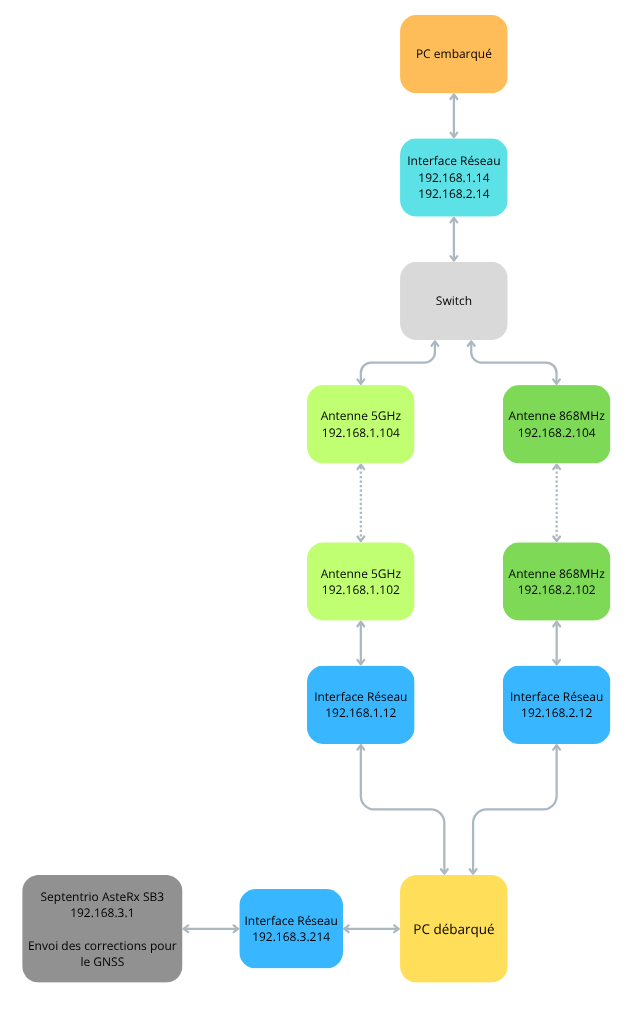
\includegraphics[width=0.7\linewidth]{Corps_rapport/PC débarqué.png}
    \captionof{figure}{Diagramme synoptique de l'architecture réseau du système}
    \label{fig28}
\end{center}
\subsubsection{Configuration et test de l'envoi d'images compressées sur l'antenne 868MHz}
L'installation double antenne étant fonctionnelle, il a alors fallu configurer le routage des différentes données sur les bonnes interfaces et automatiser à l'aide de scripts bash les opérations nécessaires au choix de l'interface à utiliser.\\\\
Une mesure de la bande passante des antennes 868 MHz a révélé que cette dernière était bien trop faible (150 ko/s) pour pouvoir transmettre l'image annotée au PC déporté. Une compression de cette dernière en h265 a alors été mise en place, divisant la bande passante nécessaire par plus de 200, la faisant passer de 17Mo/s à 80ko/s, pour une qualité à peine dégradée.\\\\
La compression h265 nécessite d'encoder l'image du côté du PC embarqué avant de l'envoyer au PC débarqué, ce qui nécessite un décodage du côté de ce dernier. \\\\
Des tests de fiabilité de la liaison ont alors été réalisés, pour comparer le réseau 5 GHz et le réseau 868 MHz, notamment sur la portée et la résilience lors de la présence d'obstacles (bâtiments et végétation dense) entre le PC débarqué et le robot.\\\\
Pour ces tests, l'envoi de l'image encodée a été fait sur chaque réseau en temps réel et le décodage a été réalisé par deux nœuds distincts. Nous avons alors pu afficher les deux retours vidéo côte à côte pour les comparer.\\\\
Les résultats obtenus montrent que l'ajout de la compression sur le retour vidéo a considérablement réduit les problèmes de communication de l'antenne 5 GHz, et que cette dernière était plus fiable, que ce soit en présence d'obstacles ou à grande distance. Nous avons alors conclu que l'ajout de l'antenne 868 MHz n'était pas nécessaire et que l'ajout de la compression ainsi qu'un choix sur les données à transmettre permettent de contrôler le robot à plus de 150 m en présence d'obstacles sans coupures, ce qui sera largement suffisant pour le défi 2.
\subsubsection{Autres tests réalisés}
D'autres tests ne rencontrant pas de problèmes particuliers ont été réalisés comme par exemple :\\
\begin{itemize}
    \item Une journée de tests à Montoldre pour tester l'ajout de la prise en compte du manque d'information dans la carte comme des obstacles au fur et à mesure que le robot s'en approche et pour évaluer les améliorations apportées par le refactoring sur la stabilité du robot lors de la conduite autonome à 3 m/s. Le seul problème noté ce jour-là était que le robot opérait de gros virages lors du retrait de l'arrêt d'urgence de sa télécommande pour lancer la conduite autonome de ce dernier. Le problème provenait du gain intégral qui commençait à s'accumuler dès lors que la conduite autonome était lancée par le téléopérateur, avant même d'avoir retiré l'arrêt d'urgence.\\
    \item Le test du mode safety first en téléopération qui ne présenta qu'un léger problème d'affichage dans l'IHM.\\
    \item Le test d'une nouvelle IHM, avec comme objectif d'évaluer l'amélioration de l'ergonomie pour qu'elle soit utilisable par une personne ne travaillant pas sur le projet. Quelques bugs mineurs ont été constatés dont un problème sur l'ajout de paramètres reconfigurables dynamiquement avec dynamic reconfigure. J'ai finalement réussi à résoudre le problème et ayant trouvé la fonctionnalité intéressante pour faciliter le paramétrage des correcteurs, j'ai modifié les briques contenant des correcteurs Pure Pursuit et longitudinaux ainsi que le correcteur de taux de lacet inclus dans l'interface du Barakuda pour ajouter la possibilité de modifier les gains dynamiquement.\\
    \item Une assistance lors des tests d'une nouvelle loi de commande avec observateurs de glissement développées par l'INRAE, qui a récemment été abandonnée car son utilisation n'était pas indispensable et que j'avais pointé une incohérence dans le protocole de tests qui était que l'on comparait pour une même trajectoire, l'écart du robot à cette dernière lors de l'utilisation de la loi de commande de l'INRAE et lors de l'utilisation du contrôleur Pure Pursuit et de la régulation longitudinale actuellement utilisés. Le problème était que la loi de commande INRAE ne fait aucune régulation de vitesse à l'approche de virages. Les résultats obtenus auraient donc été en faveur de la loi actuellement utilisée. L'utilisation de la loi de commande INRAE sera revue avec l'ajout d'une régulation longitudinale lorsque nous observerons une incontrôlabilité du robot à cause de glissements, peut-être lorsque nous monterons en vitesse.
\end{itemize}
\subsubsection{Intégration d'un planificateur global RRT*}
Enfin, en parallèle de mes tests, une tâche de fond m'a été proposée pour m'initier à la programmation en C++ lors des périodes de creux. Cette tâche consistait à reprendre un planificateur global RRT* réalisé par un ancien stagiaire l'an dernier sur la Brique MOBILEX* avant refactoring et de l'intégrer à la nouvelle version. Ce planificateur permettrait de s'affranchir de la contrainte de discrétisation du chemin liée à l'échantillonnage du MNE car les nœuds sont générés dans l'espace continu. \\\\
Le planificateur était une classe héritant d'autres classes qui avaient été modifiées lors du refactoring.\\\\
J'ai commencé par me former rapidement au concept de programmation orientée objet avec un cours d'OpenClassrooms puis j'ai pu intégrer cette classe en comparant le comportement du planificateur A* avant et après refactoring pour adapter le RRT* afin qu'il fonctionne avec les nouvelles méthodes utilisées.\\\\
Le RRT* fonctionne mais doit être modifié dans l'objectif de fournir des courbes C2, c'est-à-dire des courbes dont la dérivée seconde est continue.
\subsection{Travaux à venir}
Étant à peine plus de la moitié de mon stage, beaucoup de développements ont été réfléchis ou entamés, nécessitant des tests à venir.\\\\
En voici une liste non exhaustive :
\subsubsection{Tests de l'intégration de la détection et prise en compte des pentes et dévers}
Pour détecter et caractériser le caractère franchissable ou non des pentes et dévers, une solution consistant à se resservir du filtre de Sobel utilisé pour la détection des obstacles est envisagée, avec la particularité d'être utilisé sur une version sous-échantillonnée du MNE et avec de nouveaux seuils.\\\\
Les tests consisteront alors à s'assurer que le robot s'engage dans des pentes et dévers franchissables et contourne celles et ceux qui ne le sont pas.
\subsubsection{Tests de l'intégration de la couche sémantique dans le MNE}
Pour pouvoir intégrer les informations sémantiques dans le MNE, la solution retenue est d'attribuer à chaque point du nuage de points de la caméra une information de franchissabilité ou non. Ensuite, lors de la fusion du nuage de la caméra et du nuage LIDAR* pour mettre à jour la carte, cette information serait ajoutée aux tuiles de la carte, uniquement par les points du nuage de la caméra.\\\\
Les tests consisteront alors à vérifier que le robot puisse s'engager dans des herbes hautes.
\subsubsection{Tests de l'intégration de la couche ultrasonique dans le MNE}
Un point dur du défi 2 est la gestion des obstacles transparents car ces derniers ne sont ni détectés par le LIDAR*, ni détectés par la caméra. Une solution en cours d'évaluation serait d'utiliser les capteurs ultrasoniques pour les fusionner avec les nuages de points LIDAR* et caméra dans le MNE.\\\\
Des premiers tests ont été réalisés pour évaluer l'enveloppe de détection du capteur et la fiabilité des détections.\\\\
Les résultats obtenus montrent que le capteur pourrait nous permettre de détecter des obstacles d'au moins 50x50 cm jusqu'à 4 mètres, mais que l'orientation de ces derniers pourrait grandement affecter la distance à partir de laquelle ils seraient détectés.\\\\
Malgré ces résultats mitigés, cette solution a été retenue faute d'autres alternatives et d'autres tests seront à réaliser lors de l'ajout de cette fusion dans le MNE pour s'assurer de la bonne détection des obstacles transparents et de l'absence de fausses détections, notamment à l'approche de pentes et herbes hautes.
\subsubsection{Tests de l'impact de la fumée après modification du traitement des points LIDAR}
Pour gérer la présence de fumée, une solution jouant sur le filtrage des points LIDAR* en fonction de l'intensité a commencé à être testée et a donné des résultats prometteurs.\\\\
Des tests de l'impact de la fumée sur le nuage de points caméra et sur l'ultrason sont à réaliser maintenant que ces derniers sont également utilisés pour mettre à jour le MNE.
\subsubsection{Tests de la localisation et cartographie par SLAM}
Comme nous l'avions vu précédemment, la perte du GNSS est actuellement un point critique à résoudre car sans GNSS, la carte ne peut plus être mise à jour correctement.\\\\
Une solution en cours d'évaluation par l'Institut Pascal serait de fusionner l'odométrie fournie par le GNSS avec une odométrie fournie par un algorithme de SLAM.\\\\
Les premiers résultats obtenus sont prometteurs mais une crainte se pose sur la capacité à intégrer cette solution à la Brique MOBILEX*.\\\\
Une solution de secours qui pourrait être envisagée serait de réaliser la fusion d'odométrie non plus avec le SLAM mais avec une odométrie visuelle qui peut être fournie par la caméra.\\\\
L'évaluation de la qualité de cette odométrie m'a été demandée et est en cours. Si les résultats sont satisfaisants, je serai chargé de réaliser la fusion des odométries. La piste de fusion serait alors l'utilisation d'un filtre de Kalman* codé en Python dont la sortie alimenterait le MNE.
\subsubsection{Tests de navigation avec des pannes capteurs}
Pour continuer d'assurer le fonctionnement de la Brique MOBILEX* lors de pannes capteurs, nous avons réfléchi aux difficultés qui seront rencontrées lors de chaque panne capteur et au comportement à donner au robot dans ces conditions :\\\\
\begin{itemize}
    \item \textbf{Perte du LIDAR*} : Lors d'une perte LIDAR*, le robot continuera de mettre à jour la carte en utilisant le nuage de points de la caméra et l'ultrason. Une difficulté pourrait être rencontrée lors de la présence de fumée, où le comportement de la caméra et de l'ultrason restent à déterminer.\\
    \item \textbf{Perte de la caméra} : Comme pour une perte LIDAR*, le robot continuera de mettre à jour la carte en utilisant le nuage de points LIDAR* et l'ultrason. Le robot ne pourra cependant plus rouler dans les hautes herbes si ces dernières n'avaient pas été cartographiées avec l'information sémantique au préalable. Le robot devrait donc les considérer comme des obstacles et les contourner, ou bien s'arrêter jusqu'à la récupération de la caméra.\\
    \item \textbf{Perte du GNSS} :  Lors d'une perte GNSS, le robot doit détecter la panne pour sous-estimer la covariance du GNSS si celui-ci retourne des valeurs pour que le filtre de Kalman* priorise l'utilisation de la seconde méthode d'odométrie fusionnée (SLAM ou odométrie visuelle de la caméra).\\
    \item \textbf{Perte d'une antenne de communication} : Lors d'une perte de communication avec le PC débarqué, le robot continuera la mission en cours. Un problème de localisation pourra intervenir car les corrections de la base fixe ne seront plus envoyées au GNSS, ce qui provoquera une anomalie reprenant le comportement en cas de perte de ce dernier. Les antennes 868 MHz étant installées, une piste d'utilisation de ces dernières pour conserver l'envoi des corrections est également en cours de discussion.\\
\end{itemize}
Les autres composants ne subiront pas de pannes provoquées.\\\\
Des tests ont déjà été réalisés avec succès pour détecter la panne des capteurs ci-dessus.
\subsubsection{Tests hautes vitesses à Montoldre pour les cas du défi 2}
Lorsque l'ensemble des cas de situations du défi 2 auront été traités, des tests à haute vitesse à Montoldre seront organisés. Ces tests viseront à reproduire le plus fidèlement possible les différents scénarios auxquels nous seront confrontés le jour des épreuves.\\\\
La mise en place de ces tests m'a été confiée, notamment la réalisation des parcours reproduisant les scénarios et leur ajout dans l'IHM pour ne pas perdre de temps lors de la journée de tests.
\subsubsection{Tests des modifications du local planner}
Enfin, lors de tests de suivi de waypoints à différentes vitesses dans le simulateur, je me suis rendu compte de trois problèmes.\\\\
Le premier est que dans un cas particulier, lors d'un dégagement, le robot s'approche trop près d'un obstacle alors que la planification locale est censée exclure toute commande provoquant cette situation et qu'une fois trop près de l'obstacle, la planification ne trouve plus aucune solution. Après vérification de plusieurs hypothèses, l'hypothèse retenue serait que le modèle cinématique du robot serait imparfait, ce qui pourrait le faire dévier de la trajectoire planifiée. Cette hypothèse est confortée par l'observation de glissements du robot dans le simulateur, probablement dus à une mauvaise modélisation du contact roue/sol.\\\\
Le second intervient lors de la procédure de dégagement. Lorsque le robot, en se dégageant, trouve que la solution optimale est quasiment identique au chemin aller, il se met alors à faire des allers-retours sur place, les mêmes conditions provoquant les mêmes calculs de commande.\\\\
La résolution de ces problèmes demanderait de refaire certaines parties de la planification locale, ce qui risquerait de prendre beaucoup de temps sans garantie de résultats car le choix et le paramétrage de la fonction coût est délicat. Ces modifications ne seraient alors étudiées uniquement lorsque les autres points auront été validés.

\end{comment}